\documentclass[12pt]{graphicsclass}
\usepackage[utf8]{inputenc}
\usepackage{palatino}
\usepackage{amsmath}
\usepackage{amssymb} 
\usepackage{graphicx}
\usepackage[labelfont=bf]{caption}
\usepackage{subcaption}
\usepackage{setspace}
\captionsetup[table]{font = {stretch=1.35}}
\captionsetup[figure]{font = {stretch=1.35}}
\usepackage[margin=1in]{geometry}
\linespread{1.6}
\usepackage[hidelinks]{hyperref}
\usepackage{cite}
\usepackage{xcolor}
\usepackage{overpic}
\usepackage[all]{nowidow}

\usepackage{afterpage}
\usepackage{listings}
\usepackage{float}
\usepackage{svg}
\usepackage{url}

\usepackage{color, colortbl}
\usepackage{booktabs}

\lstdefinelanguage{JavaScript}{
  keywords={typeof, new, true, false, catch, function, return, null, catch, switch, var, if, in, while, do, else, case, break},
  ndkeywords={class, export, boolean, throw, implements, import, this},
  sensitive=false,
  comment=[l]{//},
  morecomment=[s]{/*}{*/},
  morestring=[b]',
  morestring=[b]"
}

\lstdefinelanguage{SableWasmMIR}{
  keywords={function, memory, table, global, var, const},
  ndkeywords={i32, i64, f32, f64, v128,
    int.eq, i32.const, i64.const,
    int.add, memory.guard,
    load.32, load.16,
    cast, 
    local.get, 
    call,
    local.set,
    br, br.cond, br.table, ret, phi
  }
}

\title{
{SABLEWASM: A STATIC COMPILER AND RUNTIME FOR WEBASSEMBLY}\\~\\~\\
{\large Hongji Chen, School of Computer Science \\ 
	McGill University, Montreal \\ 
	August, 2021 \\~\\~\\
	A thesis submitted to McGill University in partial fulfillment of the 
	requirements of the degree of \\~\\ Master of Computer Science }\\~\\
}

\setcounter{page}{2}\renewcommand{\thepage}{\roman{page}}

\author{\textcopyright Hongji Chen, 2021}
\date{}

\begin{document}
\maketitle


\chapter*{Abstract}
\label{sec:engAbstract}
\addcontentsline{toc}{section}{\nameref{sec:engAbstract}}
\emph{WebAssembly} is a relatively new language, introduced to improve the
performance of compute-intensive workloads in web-based applications. It offers
a compact binary bytecode intended to allow for fast compilation and improved
optimization opportunities over dynamic web languages like JavaScript. These
properties, however, also make it an interesting target for static execution,
enabling web code to run outside of a browser as well as within it. In this
thesis, we describe \emph{SableWasm}, a static, multi-pass compiler system that
translates sandboxed WebAssembly applications to native shared libraries. Our
work covers several different aspects of compiler design. First, we provide an
efficient and extensible WebAssembly module parsing and validation framework,
with improved execution speed and memory footprint compared to the reference
baseline. We then define a middle-level intermediate representation and build
an analysis and transformation framework. We explore several classic data-flow
analyses, such as dominator-tree construction within the framework, and
additionally identify several WebAssembly specific optimization opportunities,
which we address through custom transformation passes. SableWasm also
incorporates several in-progress extension proposals including the SIMD vector
operation extension. Optimized intermediate code is then converted to native
code through a backend implementation with the help of the LLVM compiler
framework and a runtime that enables C/C++ programs to interact with the
WebAssembly module directly. Finally, we evaluate SableWasm by benchmarking
against several well-known testing suites and observe performance improvement
compared to the baseline implementation.

\chapter*{Abrégé}
\label{sec:frAbstract}
\addcontentsline{toc}{section}{\nameref{sec:frAbstract}}
\begin{spacing}{1.5}
    \emph{WebAssembly} est un langage relativement nouveau, introduit pour
    améliorer les performances des charges de travail gourmandes en calcul dans
    les applications Web. Il offre un bytecode binaire compact destiné à
    permettre une compilation rapide et des opportunités d'optimisation
    améliorées par rapport aux langages Web dynamiques comme JavaScript. Ces
    propriétés, cependant, en font également une cible intéressante pour
    l'exécution statique, permettant au code Web de s'exécuter à l'extérieur
    d'un navigateur ainsi qu'à l'intérieur de celui-ci. Dans cette thèse, nous
    décrivons \emph{SableWasm}, un système de compilateur statique multi-passes
    qui traduit les applications WebAssembly en bac à sable en bibliothèques
    partagées natives. Notre travail couvre plusieurs aspects différents de la
    conception d'un compilateur. Premièrement, nous fournissons un cadre
    d'analyse et de validation de module WebAssembly efficace et extensible,
    avec une vitesse d'exécution et une empreinte mémoire améliorées par rapport
    à la ligne de base de référence. Nous définissons ensuite une représentation
    intermédiaire de niveau intermédiaire et construisons un cadre d'analyse et
    de transformation. Nous explorons plusieurs analyses de flux de données
    classiques, telles que la construction d'arbres dominants dans le cadre, et
    identifions en outre plusieurs opportunités d'optimisation spécifiques à
    WebAssembly, que nous abordons via des passes de transformation
    personnalisées. SableWasm intègre également plusieurs propositions
    d'extension en cours, y compris l'extension d'opération vectorielle SIMD.
    Le code intermédiaire optimisé est ensuite converti en code natif via une
    implémentation backend à l'aide du framework de compilateur LLVM et d'un
    runtime qui permet aux programmes C/C++ d'interagir directement avec le
    module WebAssembly. Enfin, nous évaluons SableWasm en comparant plusieurs
    suites de tests bien connues et observons une amélioration des performances
    par rapport à la mise en œuvre de base.
\end{spacing}

\chapter*{Acknowledgements}
\label{sec:ded}
\addcontentsline{toc}{section}{\nameref{sec:ded}}
First, I would like to extend my deepest gratitude to Professor Clark Verbrugge.
The work would not have been possible without his support and advice, especially
during a global pandemic. Secondly, I would like to thank Professor
Laurie Hendren for her guidance in the field of compiler design in my early days
as an undergraduate student. Finally, I would like to thank my colleagues and
friends, especially my Sable lab mates, for their encouragement throughout the
entire thesis journey.

\tableofcontents
\listoffigures %
\addcontentsline{toc}{section}{\listfigurename}
\listoftables
\addcontentsline{toc}{section}{\listtablename}

\clearpage
\pagenumbering{arabic} % restart page numbers at one, now in arabic style

%% start of chapters
\chapter{Introduction}


\section*{Contribution}

\begin{figure}
    \centering
    \includegraphics[width=\textwidth]{Images/design}
    \caption{The SableWasm compiler and runtime}
    \label{fig:design}
\end{figure}

This thesis aims to design and implement a runtime environment that enables WebAssembly to run outside of the browser. To this end, this thesis makes three major contributions. Figure~\ref{fig:design} illustrates SableWasm compiler and runtime system. We mark our contributions in the thesis as shaded boxes in the figure.

Our first contribution is a standalone WebAssembly runtime environment with support for WASI. We first start by implementing a custom extensible parser frontend for WebAssembly binary bytecode. We then define a middle-level representation for SableWasm. SableWasm MIR is a register-based control flow graph representation of the program, while, on the other hand, WebAssembly operates over a stack-based virtual machine. Hence, translating between them is nontrivial. Therefore, we design and implement a frontend code generator that lowers WebAssembly bytecode into SableWasm MIR. SableWasm MIR plays a critical role in the SableWasm system. First, it provides a middle ground where we implement an extensible and straightforward optimization framework. With the help of the framework, we experiment several analyses and optimizations on SableWasm. Second, SableWasm MIR also separates the frontend from the backend. Currently, we implement an ahead-of-time (AOT) compiler backend using the LLVM compiler infrastructure. However, there are several challenges when lowering SableWasm MIR into LLVM intermediate representation. For example, SableWasm MIR, similar to WebAssembly bytecode, utilizes abstract high-level concepts such as linear memory and indirect function call. These operations cannot be trivially mapped to LLVM instructions and requires runtime library support. Hence, the last component of SableWasm is a runtime library that provides builtin runtime functions for the generated modules and defines an easy-to-use interface for the host system.

Our second contribution in the thesis is to experiment and adopt several in-progress WebAssembly language extensions. SableWasm is designed to be extensible and currently implements four post-MVP WebAssembly features. The most interesting one among them is perhaps the fixed-width SIMD operation extension which introduces one additional value type and approximately 240 new instructions to the specification. As we have discussed earlier in this section, SableWasm MIR provides a middle ground where we perform optimization on the program. Therefore, we would like to keep the size of the SableWasm MIR instruction set simple. To achieve this goal, we carefully design a set of reduction patterns in the frontend code generator that significantly reduce the number of instructions needed. We also generalize our backend code generator that targets LLVM by emitting corresponding vector operation instructions.

Our last contribution in the thesis is to investigate how SableWasm performs and the factors that affect the performance. Here we focus on three research questions: First, how does SableWasm perform comparing to other existing WebAssembly runtime implementations? Second, does optimization over the input WebAssembly modules affect SableWasm's overall performance? Finally, does the SIMD operation extension bring performance improvement to the system? To answer these questions, we perform benchmarks against three well-known benchmark suites, Polybench \cite{polybench}, Ostrich \cite{ostrich}, and NPB \cite{npb}. We also exam generated LLVM intermediate representations in SableWasm to search for factors contributing to the slow down in the system.

\section*{Thesis outline}

This thesis consists of eight chapters in total, including the introduction chapter. Chapter 2 discusses the background information that helps the understanding rest of the thesis. It first presents the motivation for WebAssembly and WebAssembly System Interface (WASI), followed by a brief overview of the LLVM intermediate representation. Chapter 3 to chapter 5 discusses the design of implementation of the SableWasm system. Chapter 3 starts with presenting the custom extensible and efficient parser frontend for WebAssembly binary format. Chapter 4 continue the discussion of SableWasm by describing SableWasm MIR, including the code generating strategies used when lowering WebAssembly bytecode to SableWasm MIR and the optimization framework. Chapter 4 also presents several optimization passes we experimented with the framework, such as control flow graph simplification and redundant local variable elimination. Chapter 5 illustrates the last component of SableWasm, the LLVM backend and the runtime support library. In chapter 6, we investigate the performance of SableWasm by presenting benchmark results and discuss several possible theories for the slow down. Finally, chapter 7 discusses related work and chapter 8 presents our conclusion along with future work.
\chapter{Background}

This chapter provides background information that helps to understand the
thesis. We first revisit the rise of asm.js and its toolchain, Emscripten,
followed by an introduction to WebAssembly and its standardized
\emph{WebAssembly System Interface} (WASI). Finally, we will give a brief
overview of the LLVM compilation framework.

\section{Emscripten and Asm.js}

In the past decade, web-based applications are gaining popularity, and due to
the design of most browsers, programmers tend to choose JavaScript or its
dialects to implement them. One natural problem is how to compile programs that
target the native platform to run over the internet. Making the situation more
challenging, programs with a large codebase, for example games that require
complex video and physical computation, are nearly impossible to translate
line-by-line manually. In 2010, Alon Zakai started the first attempt at
translating source code that targets native platforms into JavaScript
\cite{8118483}. After two years of development, he published Emscripten that
translates LLVM intermediate representation into asm.js, a JavaScript subset
\cite{10.1145/2048147.2048224}. An asm.js program shares a similar programming
model to that which one would expect on the native platform. The detailed asm.js
specification is available on the official website
\footnote{asm.js specification: \url{http://asmjs.org/spec/latest/}}.
We will visit several critical features in asm.js with examples in
figure~\ref{fig:adler-32} (page~\pageref{fig:adler-32}). These examples are
implementations of the Adler-32 hashing algorithm used in ZLib compression
library \cite{adler32-paper} \footnote{Revisiting Fletcher and Adler Checksums:
  \\\url{http://www.zlib.net/maxino06\_fletcher-adler.pdf}}, in both C and its
corresponding generated asm.js with Emscripten.

\begin{figure}
  \centering
  \begin{subfigure}{\textwidth}
    \lstinputlisting[
      language=C,
      basicstyle=\linespread{0.4}\small\ttfamily, numbers=left
    ]{Code/adler32.c}
    \caption{C}
    \label{fig:adler-32-c}
  \end{subfigure}
  \begin{subfigure}{\textwidth}
    \lstinputlisting[
      language=JavaScript,
      basicstyle=\linespread{0.4}\small\ttfamily, numbers=left
    ]{Code/adler32.js}
    \caption{asm.js}
    \label{fig:adler-32-asmjs}
  \end{subfigure}
  \begin{subfigure}{\textwidth}
    \lstinputlisting[
      basicstyle=\linespread{0.4}\small\ttfamily,
      numbers=left
    ]{Code/adler32.wat}
    \caption{Text-format WebAssembly}
    \label{fig:adler-32-webassembly}
  \end{subfigure}
  \caption{Adler 32 in C, asm.js and text-format WebAssembly}
  \label{fig:adler-32}
\end{figure}

\paragraph{Function prologue and type annotation}
JavaScript is a dynamically typed language. Hence, a proper implementation needs
to verify the types of variables when needed. Although several optimization
techniques can eliminate some of the checks and improve the execution
performance, such language features can still incur a significant performance
loss. Asm.js adds type annotations to function parameters and expressions to
address this problem. In figure~\ref{fig:adler-32-asmjs}, Emscripten generates
parameter annotations for parameters \texttt{\$0\_1} and \texttt{\$0\_2} at
line $2$ and line $3$ respectively. The trailing bitwise `or' operation against
zero hints that both arguments are integral values since bitwise operations are
only defined for integral values in JavaScript. Emscripten also annotates
float-point numbers with the unary positive operation, `+', which we do not show
in the example. A system that supports asm.js directly can quickly recover the
type information from the annotations, which, in theory, can improve both the
compilation and execution performance. On the other hand, for a system that does
not recognize asm.js, the program above is still a valid JavaScript program, and
the type annotations ensure the correct semantics for numeric operations.

\paragraph{Control flow}
LLVM employs a register-based intermediate representation with a
\emph{control flow graph} (CFG). However, JavaScript uses structured control
flow and does not allow arbitrary jump statements similar to one would expect
in C. Hence, when translating LLVM IR to asm.js, Emscripten mimics the branch
instructions between basic blocks in the generated code with JavaScript
control-flow statements. Emscripten uses a pattern-based translation and
classifies control flow changes into three categories.
In figure~\ref{fig:adler-32-asmjs}, we demonstrate two of the three
control-flow structures, \emph{if} and \emph{loop}, at line $6$ and line $7$
respectively. Asm.js also has a third control flow structure, \emph{block},
which we do not show in the example. A \emph{block} structure is similar to a
\emph{loop} structure and can be translated to a while loop with an always-false
condition. A branch instruction referring to the \emph{block} is equivalent
to a break statement in this case. WebAssembly adopts a similar design, and we
will revisit this in the later section with more details.

\paragraph{Byte array as heap}
Emscripten uses multiple typed array views that share a single underlying byte
array buffer to simulate the heap in a native programming model.
In figure~\ref{fig:adler-32-asmjs}, the asm.js example uses \texttt{HEAPU8}, an
unsigned byte view over the byte array at line $8$, to access the data passed by
the pointer via the first argument. Asm.js also offers other array views such
as \texttt{HEAPI32} and \texttt{HEAPF32} which allows programs to access 32-bit
signed integers and single-precision floating-point numbers on the heap. This
technique also inspires the linear memory design in WebAssembly, which we will
discuss later in the chapter with more details.

Emscripten is quite successful. Experiment results show that it can port most of
the C/C++ programs of non-trivial code size to the web with approximately
50-67\% of native performance
\footnote{Alon Zakai's presentation on Emscripten at CppCon:
  \\\url{https://kripken.github.io/mloc_emscripten_talk/cppcon.html}}
without any missing significant features.

\section{WebAssembly}

Although Emscripten with asm.js is successful, there are still several problems
that remain unaddressed. One of them is the parsing overhead. As asm.js is a
strict subset of JavaScript, parsing the generated program is a non-trivial task
due to the complexity of JavaScript grammar. Additionally, because Emscripten
emits generated programs in asm.js, the output size grows significantly faster
than the native binary. Another problem regards the generated programs' safety,
especially when running an untrusted module received over the internet. In 2017,
the WebAssembly community established and proposed a new standard for
distributing programs over the internet to address these problems. The design of
WebAssembly focuses on safety, performance, portability, and compactness. The
introduction paper describes the detailed structure, validation rules
\cite{10.1145/3167082}, and execution semantics of WebAssembly
\cite{10.1145/3062341.3062363}. Here we will only visit some of the key points
that help understand the rest of the thesis. In
figure~\ref{fig:adler-32-webassembly} we also present a simple WebAssembly
program that implements the Adler32 hashing.

\paragraph{Module structure}
WebAssembly modules can have four different kinds of entities: \emph{functions},
\emph{indirect tables}, \emph{linear memories}, and \emph{globals}. Modules are
also able to import and export entities by names. In
figure~\ref{fig:adler-32-webassembly}, we define a \emph{function} and a
\emph{linear memory} and export them under name \texttt{adler32} and
\texttt{memory} respectively. WebAssembly functions can define an arbitrary
number of local variables and possibly an empty sequence of instructions as the
body. All instruction operates over an implicitly declared stack. The
control-flow will return from the function by either a \texttt{return}
instruction or reaching the end of the body. WebAssembly linear memories have
bounds consisting of a pair of integers, representing the lower bound and upper
bound respectively, \footnote{The upper bound is optional} in units of $16$-KiB
pages. In figure~\ref{fig:adler-32-webassembly}, at line $21$, we defined a
linear memory with a minimal size of $32$-KiB. WebAssembly linear memory can
also associate with zero or multiple \emph{data} segments. Each \emph{data}
segment contains a constant evaluated expression, representing the
initialization offset, and a sequence of bytes that the runtime environment will
copy from. WebAssembly indirect tables are similar to linear memories, but they
store function pointers instead of bytes. A \emph{indirect table} has a type
that consists of an upper and lower bound similar to \emph{linear memory}, as
well as a function type indicating the type of the function pointers allowed
\footnote{Currently, the function type must be \texttt{funcref} which is a union
  type of all possible function types.}. WebAssembly tables also introduce their
initializer, \emph{element} segments. The \emph{element} segment is similar to
the \emph{data} segment, but it initializes function pointers instead of bytes.
Another difference between linear memories and indirect tables is that indirect
tables are immutable after initialization to ensure the module's safety
\footnote{This is subject to change in the reference type extension}.

\paragraph{Linear memory}
Similar to asm.js, WebAssembly programs can access one or multiple
\emph{linear memories} \footnote{In the current version of WebAssembly, at most
  one linear memory is allowed within a single module}. The memory is unmanaged,
and it is the program's responsibility to handle the layout correctly. The
program can grow the \emph{linear memory} if needed via the \texttt{memory.grow}
instruction; however, the runtime environment is not obligated to increase the
\emph{linear memory}. The program can check the result of the command via the
instruction's return value. Asm.js also allows the growth of the heap byte
array. However, due to the limitations of JavaScript, this operation is usually
quite expensive, as there is no efficient \texttt{realloc} algorithm provided in
JavaScript, and it requires allocating a byte array with a larger capacity and
copying byte-by-byte. WebAssembly specification does not impose requirements on
the time complexity of growing the linear memory, yet it encourages any
implementation to avoid copying.  Unlike native heap memory, there is no
alignment requirement on load-store instructions; i.e., load-store can start at
any byte in the memory with the probable additional cost for unaligned access.
However, there are boundary checks applied to the linear memory. Any
out-of-bound access will result in a runtime panic. Additionally, WebAssembly
specification requires any runtime environment implementation to
zero-initialize the linear memory.

\paragraph{Indirect table}
Asm.js represents function pointers using first-class function values, thanks to
JavaScript. However, in WebAssembly, every entity is referred to with indices
representing references, and value types only consist of integral types and
floating-point types \footnote{WebAssembly may introduce more primitive value
  types in the future.}. Hence, we need something creative to implement the
function pointers in WebAssembly. The solution utilizes one special instruction
\texttt{call\_indirect} and indirect tables. During module initialization, the
runtime environment will initialize the indirect table according to the
\emph{element} section. Each \texttt{call\_indirect} instruction associates
with an index and an expecting type. The runtime environment will perform both
a validity check on the index and a type check with the expecting type's help.
Unlike the linear memory, the indirect table is not growable at runtime and
currently is immutable once the initialization phase is complete. An indirect
table does not limit the function pointers stored to be internal functions nor
even WebAssembly functions. The function pointer can even be a host native
function; many runtime environment implementations utilize this feature to
register native call-back functions to WebAssembly modules.

\paragraph{Structured control flow}
Another WebAssembly's key feature is the structured control structure. Unlike
the native binary and most of the bytecode representations that utilize labels
and offsets, WebAssembly has structured control flow instructions and classifies
them into three categories, \emph{block}, \emph{if} and \emph{loop}, similar to
asm.js. Each control flow instruction can optionally associate with a value
type, representing the change on the operand stack once the control block exits
\footnote{WebAssembly multivalue extension relaxes the requirement and allows
  structured control instruction to have a function type. If a control
  instruction associate with a function type, the parameter types refer to the
  value consumed from the operand stack and result types refer to the value
  added to the operand stack.}. A \emph{block} control flow is perhaps the
simplest structure. It introduces a label index to the context. The label is
only referable within the \emph{block} construct by indices. If a branch
instruction refers to the block's label, the runtime environment will redirect
the control flow as if it reaches the \emph{block}'s end. An \emph{if} control
flow is similar to the \emph{block} control flow with two significant
differences. One is that it will implicitly consume a 32-bit integer from the
stack and choose the branch accordingly. The other difference is that it can
optionally have a \emph{false} branch. If the \emph{false} branch is missing,
the runtime environment will redirect the control flow to reach the {if}'s end,
similar to the \emph{block} control flow structure. The last control flow
structure is \emph{loop}. The only difference between the \emph{loop} control
structure and \emph{block} structure is when a branch instruction refers to it.
When a branch instruction refers to a \emph{loop} block, the runtime environment
will redirect the control flow to the \emph{loop}'s beginning instead of the
end. In the figure \ref{fig:adler-32-webassembly}, we present the \emph{if}
structure on line $5$, and \emph{loop} structure on line $7$. The example does
not contain a \emph{block} structure, but there is no difference between it and
a \emph{loop} structure at the syntax level.

Generally speaking, WebAssembly's performance, compared to its native
counterpart, varies significantly from test case to test case. On the browser
side, WebAssembly can finish most test cases within $10\%$ slower than the
native version and all test cases within two times slower
\cite{10.1145/3062341.3062363}. Another test shows similar results for most
test cases, except one case is 2 times to $3.4$ times slower than native,
depending on the input size \cite{234914}. For generated code size, the
community introduction paper claims $85.3\%$ compare to native implementations.
WebAssembly is not only successful in the field of Web-based applications. It
also defines a portable format for distributing programs over the internet,
similar to what we have seen in Java and its virtual machine. GraalVM now has
its interpreter for WebAssembly modules, TruffleWasm \cite{trufflewasm}, and can
execute WebAssembly modules with impressive performance with only $4\%$ slower
than WebAssembly reference implementation in most of the cases, and even $4\%$
faster in PolybenchC.

\section{WebAssembly Extensions}

In the previous section, we presented the core part of WebAssembly published by
the community in late 2016 as a minimal viable product (MVP). Although the
WebAssembly MVP is powerful enough to host most of the applications
\cite{webassembly-survey}, there still exists room for improvement. These
post-MVP proposals enhance the functionality of WebAssembly by introducing new
instructions or modifying existing module constructs. For example, MVP
WebAssembly has no support for exception handling. Thus, when compiling programs
implemented in C++, users need to explicitly turn off the compiler's exception
feature. The exception handling post-MVP extension addresses the
problem by introducing a special \texttt{try} block which enables user-defined
stack unwinding. Most post-MVP extensions are still in the early stage of
development and may merge into core WebAssembly in the future. This project
implemented several post-MVP features such as integral value sign extension,
non-trapping floating-point conversion, multivalue semantics, and fixed-width
SIMD vector operation. In this section, we will quickly visit these post-MVP
feature extensions.

\paragraph{Integral value sign extension}
MVP WebAssembly only has 32-bit and 64-bit integral values. However, many
programming languages support integers with a smaller width. Thus, implementing
short integral values in WebAssembly is quite awkward. To alleviate the problem,
MVP WebAssembly has instructions that can perform load and store of 8-bit and
16-bit integers with signed or zero extension semantics. However, what if one
already has a short integer on the stack and would like to perform a sign
extension?  Unfortunately, there are no immediate solutions. One possible
work-around is to store the value to the linear memory and then sign extend with
the load instruction's help, which is quite expensive. The sign extension
proposal introduces new instructions that perform the sign extension for stack
values. For example, \texttt{i32.extend8\_s} consumes a 32-bit integer from the
stack then performs the sign extension to 32-bit integer operand as if the
operand is an 8-bit integer. The proposal also introduces similar instructions
for 64-bit integers.

\paragraph{Non-trapping float-to-int conversion}
MVP WebAssembly offers floating-point-to-integer conversion with implicit range
checks to fulfill the no-undefined behaviour design goal of the language. If the
desired integer type cannot accurately represent the floating-point value, the
runtime environment should trap. However, in most other languages, such as LLVM,
the conversion yields an undefined result without trapping in such scenarios.
Thus, if one wants to faithfully simulate the conversion between floating-point
and integers, an \texttt{if} block with manual checks is usually required. This
proposal introduces saturated conversion to address the problem. If the desired
integer type cannot represent the resulting number, the instruction employs
saturated semantics. More specifically, if the floating-point value is more
significant than the maximum representable value of the integer type, the
maximum value is returned, and the same holds in the case of value underflow.
This extension also lays the foundation of SIMD vector operations to achieve
more hardware-like semantics, which we will see later in this section.

\paragraph{Multivalue}
The multivalue proposal focuses on two aspects of WebAssembly, the function
return value and the types of structured-control-flow constructs. In MVP
WebAssembly, the function can have at most one return value. The proposal
generalizes the function type by allowing functions to return multiple return
values. For structured-control-flow constructs, MVP WebAssembly requires that
any instructions within the construct cannot consume stack values outside of the
stack frame. Additionally, the construct can put at most one value
onto the stack when it exists. One advantage of having such strict rules on
structured-control-flow constructs is that the validation rule is trivial, and
the runtime system can compute the stack height with minimal effort. However,
this has its drawbacks. For example, this method causes the bloat of local
variables. When entering a structured-control-flow construct, the program needs
to push all the values it may need to the local variables, then load them back
to the stack later, which is quite expensive. The multivalue proposal relaxes
such constraints by allowing the control-flow-construct to have a function type.
Function types' parameter types indicating the type of values that the construct
will consume, and the result types hint at the type of values that will be
pushed onto the stack.

\paragraph{SIMD vector operations}
Single-instruction-multiple-data (SIMD) is a powerful tool for implementing
high-performance programs. Many modern compilers, such as GCC, have
auto-vectorization analysis and transformation to automatically rewrite scalar
codes in parallel form \cite{auto-vec-gcc}. Before WebAssembly, many attempts
have been made to implement SIMD operations over the internet, most notably,
SIMD.js \footnote{\url{https://hacks.mozilla.org/2014/10/introducing-simd-js/}}.
The design of the SIMD vector operation proposal is based on the design of
SIMD.js. Currently, the proposal focuses on 128-bit vector operation, which is
widely available on different hardware architectures such as SSE
\cite{sse-intel}, and ARM Neon \cite{arm-neon}. The proposal introduces a new
value type \texttt{v128} representing a 128-bit vector. Note that the vector
type does not contain any knowledge about the element type and how to interpret
the lane, which is the number and the type of elements packed into a single
vector, depends on the instruction. The SIMD vector operations proposal takes
instructions from the intersection among different hardware architectures to
ensure the module's portability. For example, \texttt{i32x4.add} will interpret
both operands as packed 32-bit integers and perform lane-wise addition between
them, while \texttt{f64x2.sqrt} will interpret its operand as a packed
double-precision floating-point numbers. Most of the instructions are a direct
generalization of the scalar operations in MVP WebAssembly. One notable
difference is the floating-point conversion semantics. In MVP WebAssembly, the
conversion will trap in the case of overflow or underflow. In contrast, in the
SIMD vector proposal, packed floating-point value conversions follow similar
semantics to those defined in the non-trapping float-to-int conversion proposal.

\section{WebAssembly System Interface (WASI)}

In the previous section, we introduce WebAssembly as a new format for delivering
programs over the internet. Question then arises: can we push WebAssembly beyond
the browser? On the other hand, if we want to compile the native program into
WebAssembly, how do we translate operating-system-specific commands, such as
file access? Taking a step further, how do we ensure the safety of the generated
program? In the early days of development, Emscripten generates JavaScript glue
code that mimics the operating system syscalls. However, this ad-hoc solution
results in messy and nonportable code.

To address these problems, the WebAssembly community started the process of
standardizing the system interface for modules
\footnote{WASI initial announcement: \\\url{https://hacks.mozilla.org/2019/03/
    standardizing-wasi-a-webassembly-system-interface/}}. The WASI interface
design focuses on two aspects, portability and safety, following the WebAssembly
design philosophy. The interface is still under active development at the time
of thesis writing. In this project, we implement the interface functions only
if they are needed while designing the backend library to be extensible. The
official API documentation provides a detailed view on the design of the
interface \footnote{WASI API documentation: \\\url{https://github.com/
    WebAssembly/WASI/blob/main/phases/snapshot/docs.md}}.
Figure~\ref{fig:wasi-intro} gives a general illustration of the relationship
among the WebAssembly module, the runtime environment, and WASI. Here we will
focus on several key points of the design that will help understanding the
thesis.

\begin{figure}
  \centering
  \includegraphics{Images/wasi-intro.pdf}
  \caption{A illustration of WASI}
  \label{fig:wasi-intro}
\end{figure}

\paragraph{WASI ABI model}
WASI classifies modules into two categories, \emph{commands} and
\emph{reactors}. A \emph{command} module has a single entry function, namely
\texttt{\_start} and all the other exported functions are hide from the user.
On the other hand, a \emph{reactor} module has an optional initialization
function named \texttt{\_initialize}. If such initialization function is
present, the runtime environment is obligated to invoke such a function before
calling others. The runtime environment may invoke either the start or
initializer function once during a module's lifetime. Additionally, every
WASI-compatible model needs to export a linear memory under the name
\texttt{\_memory}, and all addresses referred by modules are offsets within
this linear memory. Similarly, modules will also export an indirect table
under the name \texttt{\_\_indirect\_function\_table}. The runtime environment
will pass function pointers through the indirect table. Additionally, WASI
requires the runtime environment to provide all WASI API under module name
\texttt{wasi\_snapshot\_preview1} \footnote{This will change in the future, as
  WASI is still in the standardization phase.}.

\paragraph{Sandbox}
As we described above, WASI API follows WebAssembly's design philosophy, safety,
performance, portability, and compactness. WASI modules execute under a
capability-based security system to ensure the safety of the host environment.
The host runtime system will provide a sandboxed environment for each model. For
example, for file system access, WASI standard library C works with a virtual
file system for each module with the help of libpreopen \footnote{libpreopen:
  \url{https://github.com/musec/libpreopen}} \footnote{In the more recent
  version of WASI libc, libpreopen is no longer required.}.

\paragraph{Non-invasive and extensible}
In our discussion above, one may notice that a WASI-compatible module is also a
valid WebAssembly module on its own. WASI does not introduce new instructions
nor sections to the module; instead, it provides all additional functionalities
through imported external functions. The design of WASI is also highly
extensible and split into separate modules. Currently, the WASI working group
focuses on developing the core part that provides most of the POSIX interface,
but it may add additional features in the future.

\section{LLVM Compiler Infrastructure}

In the last section of this chapter, we would like to have a quick overview of
the compiler pipeline design and LLVM compilation framework. Designing a robust
and efficient compiler in terms of both generated code and compilation speed is
challenging. The LLVM compiler framework \cite{llvm-thesis} alleviates the
problem by introducing a standardized intermediate representation (IR) between
the compiler frontends and backends. Backend developers can target their
analysis and transformations on the IR instead of specializing in different
languages. On the other hand, frontend developers can translate the source
language into the IR and expect the backend to support multiple target platforms
with efficient code generation. Figure~\ref{fig:llvm-intro} illustrates the LLVM
compilation pipeline. In this project, we are more interested in the frontend of
the framework. The LLVM official documentation and tutorial provide full details
of their intermediate representation \footnote{LLVM Language Reference Manual:
  \url{https://llvm.org/docs/LangRef.html}}. Here we will only discuss several
major differences between LLVM IR and WebAssembly that help understand the
thesis. We also provide an implementation of Adler-32 hashing in LLVM IR
generated with Clang in figure~\ref{fig:adler-32-llvm}.

\begin{figure}
  \centering
  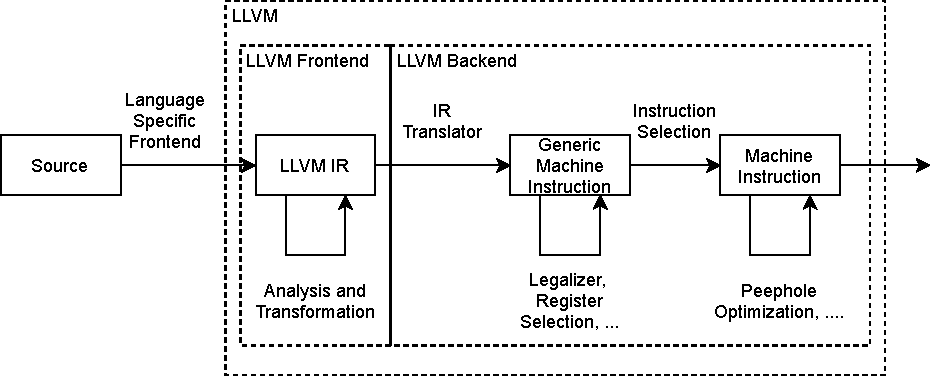
\includegraphics{Images/llvm-intro.pdf}
  \caption{A illustration of LLVM compilation pipeline}
  \label{fig:llvm-intro}
\end{figure}

\begin{figure}
  \centering
  \lstinputlisting[
    language=LLVM,
    basicstyle=\linespread{0.8}\small\ttfamily,
    numbers=left
  ]{Code/adler32.ll}
  \caption{Adler 32 in LLVM}
  \label{fig:adler-32-llvm}
\end{figure}

\paragraph{Register-based IR against stack-based IR}
In WebAssembly, all instructions operate over an implicitly declared stack. For
example, in figure~\ref{fig:adler-32-webassembly} at line $20$, a 32-bit integer
constant instruction, \texttt{i32.const}, will push the constant value on the
stack, and a 32-bit add instruction, \texttt{i32.add} will pop two values off
the stack as left-hand-side and right-hand-side operands accordingly, then push
the sum onto the stack. On the other hand, LLVM utilizes a register-based IR,
which is more similar to what one would expect on a native machine. In
figure~\ref{fig:adler-32-llvm}, each value for example, \texttt{\%0},
\texttt{\%1}, etc is a virtual register. Later in the backend, the register
allocation pass will map the virtual registers into physical registers using
register allocation algorithms.

\paragraph{Control flow, basic block, and $\phi$ instruction}
As we saw in previous sections, WebAssembly has specialized instructions to
manage the program's control flow. On the other hand, LLVM took a more
traditional approach to the problem. In 1991, researchers from IBM introduced
\emph{static single assignment} (SSA) form to ease the difficulty of writing
program analysis and transform passes \cite{ibm-ssa}. In SSA, each value has its
definition exactly once, and hence, the use-definition chain (UD chain) is
trivial to compute. The UD chain presents the relationship between variable
declarations and variable-uses in a graph. It helps the analysis pass to
efficiently pinpoint the information about variables and identify if the
variable declaration is necessary or not. However, in most of the programs,
these information needs to be merged from different control-flows; for example,
in a for-loop, the loop counter may be defined in the loop initialization and on
each loop iteration. The SSA introduces a special kind of instructions, $\phi$
instructions, which explicitly mark the merge of definitions from different
execution paths. LLVM adopts this design principle in its intermediate
representation. In figure~\ref{fig:adler-32-llvm} we have multiple $\phi$
instructions. For example, at line $11$ and $12$, value $\%7$ and $\%8$
represent $a$ and $b$ accordingly. We know that $a$ and $b$ initialized to
$0$ and $1$ upon entry and updated on each iteration from our C implementation.
In the generated LLVM IR, these merges induce $\phi$ instructions. For $a$
($\%7$), if the control flow is from the beginning of the function, we set its
value to $1$, and on the other hand, if the control flow is from the loop
iteration, we update its value accordingly. The different paths inducing a
$\phi$ instruction are indicated by basic block numbers. A basic block groups
the maximum number of instructions without control flow transfer. At line $11$,
we see the $\phi$ instruction merges the definition coming from the $\%2$
which is the entry block and $\%4$. Additionally, $\phi$ instructions must
appear before any other instructions within the same basic block, as they model
the merging of values and do not have any execution semantics.

\paragraph{Memory and load-store instruction}
The last significant difference between WebAssembly and LLVM IR is on the memory
and its related instructions. As we discussed earlier, a WebAssembly module can
have access to multiple linear memories \footnote{In the current version of
  WebAssembly, only one linear memory is allowed per module}. One might confuse
WebAssembly's linear memory with the concept of address space in LLVM IR. LLVM
IR associates each address with an integer value, namely, the address space.
However, unlike linear memory in WebAssembly, which has no difference between
one and another, the LLVM backend interprets the address space differently for
various architectures. For example, in the PTX backend, a backend target for
Nvidia GPUs, the implicit address space $0$ refers to traditional main RAM, and
address space $4$ represents the address shared by both main RAM and GPU RAM
\footnote{An introduction for PTX backend:
  \\\url{https://llvm.org/devmtg/2011-11/Holewinski_PTXBackend.pdf}}. For most
of the architecture, the implicit address space is the only address space
available to the programmer. Another difference between WebAssembly and LLVM IR
is on the design of load-store instructions. Load store instructions in both
languages have an attribute of alignment. However, LLVM IR interprets this
attribute differently from WebAssembly. In WebAssembly, the alignment attribute
acts as a hint to the runtime environment. If the alignment hint is unsuitable,
the runtime environment should still proceed under a possible penalty in the
performance. However, in LLVM IR, the alignment attribute is a requirement.
Any memory access that violates the alignment attribute will result in a
undefined behaviour, usually a runtime panic. A load-store instruction in LLVM
IR with alignment set to one will never fail. However, it will be significantly
less efficient as the backend will likely generate byte-wise load and
concatenation instructions.

We visited some of the background information that helps with understanding the
thesis in this chapter. In the next chapter, we will start from the beginning of
the system implementation, the WebAssembly parsing and validation frontend.
\chapter{Frontend}

This chapter describes the frontend of SableWasm. The front end consists of two parts, the bytecode parser and validation pass.  WebAssembly is a continuously evolving language, and its community might add new instructions in the future. Hence, the parser and the bytecode validation phase's design closely follow WebAssembly's specification and modular to ensure the framework's extensibility. A read-only view of the module structure provides additional functionality. The parser and validation phase design focuses on performance, both in execution time and memory footprint. 

\section{Bytecode Parser}
One of WebAssembly's binary format design goals is simple to parse. Although there are existing open-source bytecode parsing and validation library available when writing the thesis, such as WABT \footnote{WebAssembly Binary Toolkit: \url{https://github.com/WebAssembly/wabt.git}} provided by the WebAssembly community, there is no suitable library at the time when the project starts. Thus, for SableWasm, we implement our bytecode parsing frontend instead. The bytecode parser consists of three components, byte-source reader, WebAssembly bytecode parser and parser delegate. This section will give a brief description of each component, and figure~\ref{fig:sablewasm-parser} presents a general illustration of the parser's design.  

\begin{figure}
  \centering
  \includegraphics[width=\textwidth]{Images/sablewasm-parser.pdf}
  \caption{A illustration of SableWasm parser}
  \label{fig:sablewasm-parser}
\end{figure}

\paragraph{Byte-source Reader}
The byte-source reader consists of two parts, a byte-buffer reader and a WebAssmebly reader. The byte-buffer reader provides essential functionalities such as read and skips. Additionally, the byte-buffer reader also needs to support rewind and barrier. Any out of bound access, either beyond the barrier or byte stream exhausted, the byte-buffer reader will signal via exceptions. On the other hand, the WebAssembly reader provides a richer interface to the parser, such as decode LEB-128 encoded integers and parsing WebAssembly value types. The WebAssembly reader is also responsible for validating the result before passing it to the parser. In the case the result is invalid, the reader throws exceptions similar to the byte-buffer reader.

\paragraph{WebAssembly Parser}
WebAssembly parser is the kernel part of the parsing framework. As we discussed earlier in the chapter, one of the primary design goals of the framework is its extensibility. Hence, the SableWasm parser is modular and consists of three parts, parser core, custom section parser and instruction extension parser. The grammar for WebAssembly binary representation is quite simple, and hence, the parser core implements a simple top-down recursive descent parser with a single byte look-ahead.

\emph{Custom sections} are a special section defined in the WebAssembly standard. They are essentially a binary data chunk tagged with a string name. How to interpret the binary data is different from one to another. These custom sections can either be standardized by the community or defined specific to a toolchain. In this project, we implement two custom sections standardized by the WebAssembly working group, namely \emph{Name} section and \emph{Producer} section. The \emph{Name} section gives human-readable names to functions and their local variables that help program debugging. The specification does not require these names to be the same as the import or export names. There is no direct support for more detailed debug information encoding in WebAssembly, at the time of thesis writing. However, extensions are working on this problem, such as DWARF for WebAssembly \footnote{DWARF for WebAssembly: \url{https://yurydelendik.github.io/webassembly-dwarf/}}; on the other hand, the \emph{Producer} section is relatively simple. It only encodes the information about the toolchain that generates the module, such as the toolchain name and version. All custom section parsers in SableWasm derived from the base class \texttt{CustomSection}. The parser core will dispatch the binary chunk to search custom section parser based on the name tag. Each custom section parser manages its results and does not communicate to the parser delegate directly. Instruction extension parsers focus on another different aspect of the WebAssembly module.

In the background section, we have visited several extensions that merged to the WebAssembly specification. A quick reminder, WebAssembly extensions can insert or modify the instructions defined in the minimum-viable-product (MVP)  specification. The SableWasm WebAssembly parser employs instruction extension parsers to address this problem. When the parser intends to parse an instruction, it will iterate over all its instruction extension parsers in a chained manner. If the instruction opcode is not recognized by any registered instruction extension parser nor in the minimum-viable-product specification, the parser will signal the error by throwing an exception. 


\section{WebAssembly Bytecode Representation}

\section{WebAssembly Bytecode Validation}

\section{Performance Evaluation}
\chapter{Middle-level Intermediate Representation}

\section{MIR Design}

\subsection{MIR Module Entities}

\subsection{MIR Instructions}


\section{Translating WebAssembly to MIR}

\subsection{Structured-Control-Flow Construct}

\subsection{Instructions Reduction}

\section{Analysis Framework}

\subsection{Type Infer}

\subsection{Dominators and Dependence}

\subsection{Local Value Numbering}

\subsection{Control-Flow Graph Simplification}

\subsection{Redundant Local Variable Elimination}

\chapter{Backend and Runtime}
\label{chapter:backend-and-runtime}

This chapter discusses the last component of the SableWasm compilation pipeline:
the code generation backend and runtime support for generated shared libraries.
Currently, SableWasm has only one backend based on the LLVM compiler
infrastructure. However, in the future, one can easily extend the system by
adding more backends that lower SableWasm MIR into other target languages.
Another problem that appears when designing a backend is how SableWasm MIR
entities map to native constructs. In SableWasm, we take an instance-based
approach. The SableWasm runtime library will manage all entities in an instance
object. The system will pass it to the generated native functions as the first
argument, similar to `this' pointer in many C++ implementations. In the rest of
this chapter, we will first go through the design of the instance object,
followed by the implementation of WebAssembly entities. Finally, we will
discuss the code generation strategies used when lowering SableWasm MIR to LLVM
intermediate representation and the interaction between generated shared
libraries and the hosting language.

\section{Instance Layout}

\begin{figure}
    \begin{minipage}{.35\textwidth}
        \centering
        \includegraphics[
            width=\textwidth
        ]{Images/5.Backend and Runtime/instance}
    \end{minipage}\hfill
    \begin{minipage}{.6\textwidth}
        \begin{lstlisting}[
            language=C, 
            basicstyle=\linespread{1}\ttfamily\footnotesize]
struct instance {
    memory_metadata_t   *memory_metadata;
    table_metadata_t    *table_metadata;
    global_metadata_t   *global_metadata;
    function_metadata_t *function_metadata;
    memory_t            *memories[NUM_MEMORY];
    table_t             *tables[NUM_TABLE];
    global_t            *globals[NUM_GLOBAL];
    struct {
        struct instance *context;
        function_t      *function_ptr;
    } *functions[NUM_FUNCTIONS];
};        
    \end{lstlisting}
    \end{minipage}
    \caption{SableWasm WebAssembly instance}
    \label{fig:backend-instance}
\end{figure}

This section discusses the WebAssembly instance implementation in SableWasm.
A WebAssembly instance hosts all the runtime structures that the generated
shared libraries require, such as linear memories and indirect tables.
Figure~\ref{fig:backend-instance} illustrates the design of the WebAssembly
instance. SableWasm's WebAssembly instance object consists of two parts,
metadata entries and entity pointers. One may also notice that the instance
object's size may vary from one module to another depending on how many entities
are declared. This behaviour is intentional by design. The SableWasm runtime
system needs to compute the address of the pointers based on the metadata
information on the fly. By packing all pointers in a consecutive memory region,
we reduce one layer of indirection for the runtime system, and in theory, may
improve runtime performance. On the other hand, the generated shared library
has all the entities address inlined as the backend can compute them during code
generation, which does not incur any performance loss. For most of the entities,
they are pretty straightforward, and we will skip the discussion here. In the
rest of the section, we focus on three aspects: the metadata entries,
the function entity representations, and the instance initialization protocol
in SableWasm.

\paragraph{Metadata}
One could think of the metadata as the signatures for entities, and indeed, the
SableWasm runtime system prepares the instance object based on the metadata.
Further, shared libraries generated by SableWasm only publicly expose the
metadata and initialization function to conceal module details. Metadata encodes
the type for the entity. For linear memories and indirect tables, this is
relatively trivial as their types only consist of an integer pair. In the case
of global variables, things are a little bit complicated. A quick reminder,
WebAssembly global variable types keep track of their value type and mutability.
The first problem here is how to encode WebAssembly value types. One solution is
to use WebAssembly value type binary format. However, this encoding strategy is
hard to maintain as a human cannot directly read them. Here we use the JVM
approach for value type encoding
\footnote{\url{https://docs.oracle.com/javase/7/docs/technotes/
        guides/jni/spec/types.html}}. In short, in SableWasm, we encode
32-bit integers as `I', 64-bit integers as 'J', single-precision floating-point
numbers as 'F', double-precision floating-point numbers as 'D', and finally,
128-bit vectors as 'V'. The second problem is how to encode mutability. In
SableWasm, we use capital letters for constant global variable types and lower
letters for mutable ones. Finally, for function types, we follow a similar
design as we used for global variables. SableWasm encodes a function type into a
null-terminated string. Let's take \texttt{[i32, f32] -> [v128]} as an example.
SableWasm encodes the type into `\texttt{IF:V}'. The colon acts as a separator
between parameter types and result types. Note that `\texttt{:}' itself is also
a valid SableWasm function signature string, and represents \texttt{[] -> []},
a void function with no arguments. Finally, metadata also encodes module names
and entity names for import entities and names for export entities, which play
a critical role later in the module initialization phase.

\paragraph{Function entity representation}
The WebAssembly specification classifies the functions into two groups,
WebAssembly functions and host functions. WebAssembly functions are any
functions defined within a WebAssembly module. On the other hand, host
functions are directly provided by the host system, and from the WebAssembly
module's perspective, the host functions are black boxes without any knowledge
of their internals. Making things more complex, in MVP WebAssembly, there are no
explicit requirements on how the WebAssembly functions should behave if they
are invoked from other modules. Here we use a similar generalization like the
one adopted by Javascript \footnote{WebAssembly Javascript Interface:
    \url{https://www.w3.org/TR/wasm-js-api-1/}}. In short, in SableWasm, if a
module exports a function, it exports the function in a closure that captures
its enclosing instance. Suppose a second module invokes the exported closure
as an import function. In this case, the function still only has access to its
original module's entities and only communicates to the second module via
return values. Hence, in SableWasm, we implement our function as a pair of
pointers. The first one refers to its enclosing instance, and the second one
relates to the generated function code. In this chapter's introduction, we
mentioned that we pass the instance object as the first argument to the
generated functions upon function calls. But, what should we give to the host
function invocations? SableWasm defines that for all the host functions, the
instance object pointer will always point to the caller's enclosing instance
so that the host functions can access the internals of the caller's module.

\paragraph{Initialization protocol}
In the last part of the section, we will cover the initialization protocol we
used in SableWasm. The initialization protocol consists of three basic steps:
validation, instance preparation, and initialization.
In the validation phase, we load the shared library with the operating system's
help, such as \texttt{dlopen} on Linux, and check if it contains all the
required symbols. Currently, a SableWasm shared library needs to export five
symbols in total. Table~\ref{tbl:sablewasm-runtime-export-syms} illustrates the
symbols expected from the generated shared libraries. The instance initializer
function takes a \emph{prepared} instance object as the argument. The next step
in SableWasm is to construct this \emph{prepared} instance object. The idea of
a \emph{prepared} instance object is that we want to separate the memory
allocation from the value initialization. In SableWasm, the runtime system
handles the memory allocation, while on the other hand, the initializer function
takes care of the value initialization. In the second phase, the SableWasm
runtime allocates all the entities and attaches them to the module instance.
Note that SableWasm also resolves all the import names at this stage, and it
will only proceed to the next step if all the expecting import entities are set.
The import name binding utilizes the module names and entity names provided by
the metadata. Finally, the last step is the initialization. SableWasm will
invoke the initializer function supplied by the shared library. The initializer
function takes care of all kinds of value initialization, such as setting values
for global variables and copying data segments into linear memories. If the
runtime system adequately prepares the instance context, the initializer
function should never fail.

\begin{table}[h]
    \centering
    \begin{tabular}{|l|l|}
        \hline
        \textbf{Symbol Name}          & \textbf{Description}          \\ \hline
        \_\_sable\_global\_metadata   & Metadata for global values    \\ \hline
        \_\_sable\_memory\_metadata   & Metadata for linear memories  \\ \hline
        \_\_sable\_table\_metadata    & Metadata for indirect tables  \\ \hline
        \_\_sable\_function\_metadata & Metadata for functions        \\ \hline
        \_\_sable\_initialize         & Instance initializer function \\ \hline
    \end{tabular}
    \caption{SableWasm shared libraries exported symbols}
    \label{tbl:sablewasm-runtime-export-syms}
\end{table}
\section{WebAssembly Entities}
\label{section:runtime-webassembly-entities}

In the previous section, we discuss the design of the SableWasm WebAssembly
instance object. However, we treat all WebAssembly entities as opaque pointers
without diving into the details during the last section. This section will cover
the implementation of the WebAssembly entities along with the runtime library
builtin functions in SableWasm. Before we start this section, we will first
present the terms used throughout the later part of the thesis. In the rest of
this chapter, we use \texttt{\_\_sable\_instance\_t} to denote the type of the
instance object. Similarly, we use a similar format when discussing WebAssembly
linear memories, indirect tables, and global variables. For example,
\texttt{\_\_sable\_memory\_t} is the type of WebAssembly linear memory in
SableWasm. Finally, we use \texttt{\_\_sable\_function\_t} refer to the function
pointers that point to generated native functions.

\paragraph{Linear Memory}

\begin{figure}
    \centering
    \includegraphics[width=0.85\textwidth]{Images/5.Backend and Runtime/memory}
    \caption{SableWasm WebAssembly linear memory}
    \label{fig:backend-memory}
\end{figure}

SableWasm implements WebAssembly linear memories with mapped memory provided
by the operating system. It also has a fallback implementation that uses
standard \texttt{malloc} and \texttt{free} procedure from the C library for an
operating system that does not support mapped memory. The fallback
implementation is relatively trivial, and we will not discuss it in the thesis.
Here, we will focus on the one that uses mapped memory.
Figure~\ref{fig:backend-memory} illustrates the strategies when mapping
WebAssembly linear memory into native memory. On the top, we have a linear
memory with a size of 1 in WebAssembly page size units, or 64KiB. In the figure,
we assume the native machine has a page size of 4KiB, which is typical for most
hardware architectures. Here's a quick recap on the requirements of WebAssembly
linear memories. First, the program can efficiently random access any location
within the linear memory. Second, at runtime, the module can query
the size of the linear memory. Finally, the program can grow the linear memory
if the runtime system allows it. SableWasm implements linear memories using
a similar trick as the one used for `\texttt{malloc}' functions in many C
standard library implementations. From the generated shared libraries'
perspective, the linear memory object points to the start of a continuous
memory chunk. Hence, memory accesses are efficient and require only one layer
of indirection. First, the generated function will fetch the linear memory base
pointer from the instance object and calculate offsets accordingly.
SableWasm also attaches an extra page that manages the metadata of the linear
memory at the beginning. It contains all the records that the runtime system
needs to work with the linear memory, such as the current size and the upper
bound. Note that the size of the metadata is usually way smaller than the page
size defined by the native machine. Still, SableWasm reserves a whole page for
it, as we want our linear memory start address to be always page-aligned in the
hope of better performance.

\begin{table}[h]
    \centering
    \begin{tabular}{|l|l|}
    \hline
    \textbf{Runtime builtin functions} & \textbf{Description}                              \\ \hline
    \_\_sable\_memory\_size            & Query for the size of the linear memory           \\ \hline
    \_\_sable\_memory\_guard           & Perform boundary check on the linear memory       \\ \hline
    \_\_sable\_memory\_grow            & Attempt to increase the size of the linear memory \\ \hline
\end{tabular}
    \caption{SableWasm runtime builtin functions for linear memory}
    \label{tbl:sablewasm-runtime-memory-api}
\end{table}

SableWasm implements additional functionalities through library functions.
Table~\ref{tbl:sablewasm-runtime-memory-api} illustrates all runtime library
builtin functions provided by SableWasm. \texttt{\_\_sable\_memory\_size}
implements SableWasm's \texttt{MemorySize} instruction. It takes an argument of
a linear memory instance and returns the size of it in WebAssembly page units.
The second runtime builtin function, \texttt{\_\_sable\_memory\_guard}
corresponds to the \texttt{MemoryGuard} instructions in SableWasm. It takes
a linear memory instance and the expected number of bytes ahead as arguments.
Note that the function does not return any values, and this is intentional
by design. SableWasm runtime library utilizes the C++ exception mechanism to
report and handle errors. If the memory access is out-of-bound, the runtime
system will throw an exception. We will come back to this later in this chapter
when discussing the interaction between generated shared libraries and the
host language. Finally, the last runtime builtin function,
\texttt{\_\_sable\_memory\_grow} implements the SableWasm's \texttt{MemoryGrow}
instruction. The instruction follows its counterpart that appeared in the
WebAssembly specification. It takes a linear memory instance and the number of
pages to increase as arguments. If the operation is successful, the function
will yield the new size of the linear memory; otherwise, it returns -1 instead.
SableWasm grows the memory by remapping the memory with the help of the
operating system. On Linux, this usually corresponds to a
\texttt{mremap} operation.

In the above implementation, all linear memory bounds checks are explicit and
program-directed, and thus they are relatively quite expensive. To further
improve the performance, we use a similar technique to that used by many
virtual machine implementations, which utilizes mapped memory access permission
flags. Figure~\ref{fig:backend-memory} illustrates this approach at the bottom.
One may notice that MVP WebAssembly works with 32-bit addressing
\footnote{This is subject to change in the future.
    WebAssembly 64-bit memory addressing:\\
    \url{https://github.com/WebAssembly/memory64}}. Hence, the maximum size of
the linear memory is 4GiB. Thus, SableWasm reserves 4GiB of address when
allocating a linear memory and marks all the pages beyond the current range as
invalid pages. This operation is quite efficient as it only works with the
memory address instead of allocating the memory. In this implementation, any
out-of-bound access will result in a memory segmentation fault. Note that this
strategy does yield better performance but results in a non-recoverable error.
SableWasm provides both implementations, and one can select based on their
needs. In the next chapter, when we compare SableWasm's performance against
several other implementations, we always use the second strategy, as the
recoverable code is not required.

\paragraph{Global}

\begin{figure}
    \centering
    \includegraphics[width=\textwidth]{Images/5.Backend and Runtime/global}
    \caption{SableWasm WebAssembly linear global}
    \label{fig:backend-global}
\end{figure}

Compared to the WebAssembly linear memory implementation, SableWasm's
WebAssembly global variable implementation is relatively straightforward. In
the current version of WebAssembly, global variables can only store primitive
values. Therefore, SableWasm holds the WebAssembly global variable instance as
a union construct of all possible value types, followed by its type's character
encoding. Figure~\ref{fig:backend-global} illustrates SableWasm's implementation
for WebAssembly global variable instances. From the generated shared libraries'
perspective, the global variable access is equivalent to a simple load or store
operation. Note that, in generated shared libraries, we never need to worry
about the mutability of the global variables because the WebAssembly validation
rules ensure that a valid module should never write to a constant global
variable.

\paragraph{Indirect Table}
The last WebAssembly entity implemented in SableWasm is the indirect table, and
it perhaps is the most complex one among all three of them. A quick reminder,
in the instance layout section, we mentioned that we represent the function
instance in SableWasm using function closures that capture its enclosing
context. SableWasm implements the indirect table using a vector of function
closures and their type signatures. The internals of the SableWasm indirect
table is hidden from the generated shared libraries and only communicates to
them via runtime buitlin functions. Table~\ref{tbl:sablewasm-runtime-table-api}
illustrates all the runtime builtin functions provided by SableWasm for
indirect tables.

\begin{table}[h]
    \begin{tabular}{|l|l|}
    \hline
    \textbf{Runtime builtin functions} & \textbf{Description}                                        \\ \hline
    \_\_sable\_table\_guard            & Check if a given index is within the indirect table's range \\ \hline
    \_\_sable\_table\_check            & Check if the entry has specific type                        \\ \hline
    \_\_sable\_table\_context          & Fetch the context pointer of the entry                      \\ \hline
    \_\_sable\_table\_function         & Fetch the function pointer of the entry                     \\ \hline
    \_\_sable\_table\_set              & Write to indirect table                                     \\ \hline
\end{tabular}
    \caption{SableWasm runtime builtin functions for indirect table}
    \label{tbl:sablewasm-runtime-table-api}
\end{table}

\texttt{\_\_sable\_table\_guard} takes the indirect table instance and the
index as arguments. It is quite similar to \texttt{MemoryGuard} instructions,
except that it works with an indirect table. In addition, it also utilizes the
same error handling strategy by throwing an exception in the case where the
index is out-of-bounds. The next runtime builtin function,
\texttt{\_\_sable\_table\_check} implements the runtime type checking for
indirect function calls. It takes a pointer to an indirect table instance,
an index, and a function signature string as the parameter. We use the same
strategy as we have seen in the instance layout section to encode the
expecting type of the function. As in the current SableWasm, the type system is
extremely trivial, there is no complex typing judgment involved, such as
subtyping. Hence, the runtime type checking for indirect function calls is just
a simple string comparison. In the case of type mismatch, the runtime type
checking function also throws an exception. \texttt{\_\_sable\_table\_context}
and \texttt{\_\_sable\_table\_function} are the getter functions provided by
SableWasm. Both of them take an indirect table instance and an index as the
argument. These two functions assume the access is within range, and the
indirect table entry has the expected function type. We will come back to this
later in the chapter when we discuss the patterns used when lowering SableWasm
MIR into LLVM intermediate representations. As their names suggest, the first
function returns the pointer to the context instance object, and the second
function returns the function code address. Finally, the last runtime builtin
function for indirect tables is \texttt{\_\_sable\_table\_set}. Although in MVP
WebAssembly, indirect tables are immutable, the program cannot alter them after
they initialized \footnote{This is subject to change in the future. WebAssembly
    reference types:\\\url{https://github.com/WebAssembly/reference-types}},
the module initialization function still needs the setter function to setup
WebAssembly element segments. The setter function takes an indirect table
instance, an index, a function code address, and its null-terminated type
signature string as the argument. Similar to the getter functions, the setter
function assumes the index is always within range.

The SableWasm runtime library still provides another runtime builtin function
that does not fit into the categories above. SableWasm MIR defines an
\texttt{Unreachable} instruction, which should never reached by any control
flow, and if so, it will signal a runtime panic. In many other languages,
\texttt{Unreachable} maps to a hardware trap instruction, such as \texttt{ud2}
instruction on x86 architecture. However, this behaviour is not acceptable in
SableWasm. \texttt{ud2} generates a non-recoverable hardware invalid instruction
exception, which will eventually lead to the entire system core dump; on
the other hand, SableWasm expects exceptions thrown from generated shared
libraries and should handle them accordingly. Hence, the SableWasm runtime
library provides the \texttt{\_\_sable\_unreachable} function for the SableWasm
MIR \texttt{Unreachable} instruction. We will come back to this with more
details in the following section when discussing the code generation strategy
used when lowering SableWasm MIR into LLVM intermediate representation.
\section{Code Generation}
\label{section:runtime-codegen}

This section describes the code generation strategy used in the SableWasm LLVM
backend. For most of the instructions, especially for SableWasm MIR numeric
operations, the translation rules are simple mappings between SableWasm MIR
instructions and their LLVM counterparts. In this section, we will skip the
discussion over these trivial mapping. Instead, one can consult the SableWasm
source code for more details. The rest of the section will focus on several
key aspects: local variable implementation, linear memory manipulation,
indirect function calls, and SIMD instruction operations. One problem that
arises when lowering SableWasm MIR into LLVM intermediate representation is
how to pick the instruction translation order. Any instruction in SableWasm MIR
can refer to values either generated by a previous instruction in the same basic
block or instructions within a dominating block, implying that when lowering
SableWasm MIR, we need to perform a pre-order tree traversal over the dominator
tree. However, $\phi$ nodes may exist merging candidate values from prior
dominating blocks or due to subsequent backward branching.
Hence, the translation visitor may not have translated the candidate value
before $\phi$ nodes. SableWasm backend takes a two-phase translation to address
this problem. In the first pass, the backend will translate all the instructions
and collect the resulting values into a map, and in the second pass, the backend
will come back to the $\phi$ nodes and fix up the candidate values accordingly.

\paragraph{Function declaration and local variables} \quad
\begin{lstlisting}[
  basicstyle=\linespread{1}\small\ttfamily, 
  language=LLVM, 
  mathescape=true]
function %foo: [i32] -> [f32] {
  {(arg) %local0: i32, %local1: f64} 
  ......
}
$\Longrightarrow$
define private float @foo(%__sable_instance_t* %0, i32 %1) {
entry:
  %2 = alloca i32, align 4
  store i32 %1, i32* %2, align 4
  %3 = alloca double, align 8
  store double 0.000000e+00, double* %3, align 8
  ......
}

{%local: i32} 
%t0 = local.get %local $\Longrightarrow$ %t0 = load i32, i32* %local, align 4
local.set %local %t0 $\Longrightarrow$ store i32 %t0, i32* %local, align 4
\end{lstlisting}

We will first start by examining the translation pattern for lowering SableWasm
MIR functions into LLVM functions and their local variables. The example above
presents a simple function named \texttt{foo}, which takes a single 32-bit
integer as the argument and returns a single-precision floating-pointer number.
\texttt{foo} has two local variables. The parameter implicitly introduces the
first one, \texttt{local0}, and the function explicitly defines the second one,
\texttt{local1}. At runtime, \texttt{local0} will hold the value of the
parameter upon entry, and \texttt{local1} will initialize to zero. Compared to
the SableWasm MIR function definition, the one in LLVM intermediate
representation (IR) has three major differences. First, the LLVM function
definition has the extra instance object pointer in the arguments, in the
example above, \texttt{\%0}. We covered this briefly in the instance layout
section. In short, for all the functions, the SableWasm backend code generator
will implicitly add the instance object pointer as the first argument. The
second difference is in the entry block. SableWasm MIR, similar to WebAssembly,
views the local variables as opaque memory slots. However, LLVM IR requires
users to manually allocate them in stack memory space via the \texttt{alloca}
instruction. The \texttt{alloca} instruction reserves enough memory on the
stack based on the given type and returns a pointer. In example above,
\texttt{\%2} and \texttt{\%3} are two reserved local variable memory region
that correspond to \texttt{local0} and \texttt{local1} accordingly. The last
difference is that SableWasm IR defines implicit initialization for all local
variables; on the other hand, LLVM \texttt{alloca} instruction leaves the
reserved memory with uninitialized values. Hence, to faithfully implement
WebAssembly and SableWasm MIR specification, we generate \texttt{store}
instructions to set the initial values for each local variables. As for
\texttt{LocalGet} and \texttt{LocalSet} instructions, the translation patterns
are quite straightforward. The SableWasm backend code generator maps
\texttt{LocalGet} instructions to \texttt{load} instructions and
\texttt{LocalSet} instructions to \texttt{store} instructions as demonstrated
in the example above.

\paragraph{Linear memory operation} \quad
\begin{lstlisting}[
  basicstyle=\linespread{1}\small\ttfamily, 
  language=LLVM, 
  mathescape=true]
$\text{\textbf{Fetching linear memory:}}$
%t0     = getelementptr 
            inbounds %__sable_instance_t, %__sable_instance_t* %0, 
            i32 0, i32 4
%memory = load %__sable_memory_t*, %__sable_memory_t** %t0, align 8

%t0 = memory.size %mem $\Longrightarrow$
%t0 = call i32 @__sable_memory_size(%__sable_memory_t* %mem)
%t0 = memory.grow %mem %delta $\Longrightarrow$
%t0 = call i32 @__sable_memory_grow(%__sable_memory_t* %mem, i32 %delta)
memory.guard %mem %offset $\Longrightarrow$
call void @__sable_memory_guard(%__sable_memory_t* %mem, i32 %offset)
\end{lstlisting}
In section~\ref{section:runtime-instance-layout} and
\ref{section:runtime-webassembly-entities}, we presented how the
instance object manages the linear
memory instance and several runtime functions that implement additional
functionalities. The SableWasm backend code generator takes advantage of the
design by mapping SableWasm linear memory manipulation instructions into builtin
function invocations. The example above demonstrates the mapping for
\texttt{MemorySize}, \texttt{MemoryGrow} and \texttt{MemoryGuard} instructions.
All these instructions map to \texttt{call} instructions to their corresponding
builtin functions with appropriate arguments. Note that all builtin functions
require passing the linear memory pointer as an argument. Currently, the
WebAssembly module can have at most one linear memory. Due to the validation
rules, such linear memory must present within the module if linear memory
manipulation instructions appear in the program. Further, as we store linear
memory instance pointers before any other entities, one can show that the
linear pointer must be the 5th pointer in the instance object. Hence, the
SableWasm backend code generator fetches the linear memory instance pointer
using a pair of a \texttt{getelementptr} instruction and a \texttt{load}
instruction. The \texttt{getelementptr} instruction LLVM calculate addresses
for entries in a aggregation. The above example calculates addresses base on
the type \texttt{\_\_sable\_instance\_t} which is generated according to
declared entities at compile time.

\paragraph{Linear memory load and store} \quad
\begin{lstlisting}[
  basicstyle=\linespread{1}\small\ttfamily, 
  language=LLVM, 
  mathescape=true]
$\text{\textbf{Load a 32-bit integer:}}$
%result = load.32 i32 %mem %addr $\Longrightarrow$
  %t0     = ptrtoint %__sable_memory_t* %memory to i64
  %t1     = zext i32 %offset to i64
  %t2     = add nuw i64 %t0, %t1
  %addr   = inttoptr i64 %t2 to i32*
  %result = load i32, i32* %addr, align 1
$\text{\textbf{Partial load a 32-bit integer:}}$
%result = load.16 i32 %mem %addr $\Longrightarrow$
  ......
  %t0     = load i16, i16* %addr, align 1
  %result = zext i16 %t0 to i32
$\text{\textbf{Store a 32-bit integer:}}$
store.32 %mem %addr %val $\Longrightarrow$
  ......
  store i32 %val, i32* %addr, align 1
$\text{\textbf{Partial store a 32-bit integer:}}$
store.16 %mem %addr %val $\Longrightarrow$
  ...... 
  %t0    = trunc i32 %val to i16
  store i16 %t0, i16* %addr, align 1
\end{lstlisting}
SableWasm MIR classifies load and store instructions into two groups,
partial and complete. A quick reminder, WebAssembly associates load and store
operations with sign extension mode, while in SableWasm, we define load
instruction to perform zero extension, and store instructions always apply bit
truncation. The first example above presents a complete load operation for a
32-bit integer. The translation pattern is relatively straightforward. Note
that the linear memory instance pointer points to the first byte within the
linear memory. Hence, the SableWasm backend code generator will first calculate
the native write address by summing up offset and base pointer and map the
\texttt{Load} instruction to \texttt{load} in LLVM. The LLVM memory operation,
such as \texttt{load} and \texttt{store} has a complementary attribute,
\texttt{align}. In the background section, we introduced the attributes in
LLVM. In short, the \texttt{align} attribute marks an alignment requirement for
memory access operations. As WebAssembly linear memory is comparable to a byte
array, in which read-write can occur at any point, we can only conservatively
set the alignment to one in order to limit the LLVM backend instruction selector
from generating instructions with alignment assumptions. This, in theory, leads
to less efficient code. However, later in the evaluation section, we determine
this is not a bottleneck of the entire implementation. In the future, one can
further improve the performance of SableWasm by designing analyses that infer
lower bounds for alignment. The second example above demonstrates the
translation pattern for partial load operation. Compared to the complete load
instruction, the translation pattern for partial load instruction has an
additional zero-extending operation, \texttt{zext} at the bottom, to implement
the SableWasm MIR partial load semantics. On the other hand, the translation
pattern for both complete and partial \texttt{store} instructions are very
similar to \texttt{load} instructions. The most notable difference is the
\texttt{trunc} instruction in partial \texttt{store}'s translation pattern
which performs bit truncation on the operand.

\paragraph{Indirect function call} \quad
\begin{lstlisting}[
  basicstyle=\linespread{1}\small\ttfamily, 
  language=LLVM, 
  mathescape=true]
call.indirect %table %index %expect_ty $\Longrightarrow$ 
  call void @__sable_table_guard(%__sable_table_t* %table, i32 %index)
  call void @__sable_table_check(
    %__sable_table_t* %table, i32 %index, i8* %expect_ty)
  %t0 = call %__sable_instance_t* @__sable_table_context(
    %__sable_table_t* %table, i32 %index)
  %t1 = call %__sable_function_t* @__sable_table_function(
    %__sable_table_t* %table, i32 %index)
  %t2 = icmp eq %__sable_instance_t* %t0, null
  %t3 = select i1 %t2, %__sable_instance_t* %0, %__sable_instance_t* %t0
  %t4 = bitcast %__sable_function_t* %276 to ......
  %t5 = call ...... %t4(%__sable_instance_t* %t3, ......)
\end{lstlisting}
The SableWasm backend code generator implements indirect function calls via a
series of builtin function invocations. We have already presented the builtin
function in section~\ref{section:runtime-webassembly-entities}; hence, we will
not show them in detail in this
paragraph. The first step for calling an indirect function is to check if the
index is within range by calling the \texttt{\_\_sable\_table\_guard} builtin
function. If the index is within range, we then compare the expected function
type with the actual indirect function type with
\texttt{\_\_sable\_table\_check}. Note that this builtin function also checks
if the entry is a null function. If so, it will report an exception. The
SableWasm backend code generator uses a similar technique to encode the
expected function type into a null-terminated string, as we have seen in
section~\ref{section:runtime-instance-layout}. After we make sure the indirect
function is valid, we can now
fetch the context pointer and function address pointer by using two getter
functions, \texttt{\_\_sable\_table\_context} and
\texttt{\_\_sable\_table\_function}. Before we invoke the function, we need to
check if it is a host function. A quick reminder, SableWasm will set context
pointers for all host functions as null pointers, and when invoking a host
function, we need to pass the current instance object pointer as the context
pointer. The SableWasm code generator chooses the correct context pointer by
using a pair of \texttt{icmp} and \texttt{select} instruction. After selecting
the correct context pointer, the indirect function is straightforward by
casting the function code address into the function pointer and invoking it
appropriately. One may notice that the indirect function call in SableWasm is
costly and involves multiple function calls. WebAssembly specification does not
impose requirements on indirect function call efficiency, and later in our
benchmark, we determine that indirect function calls are not a performance
bottleneck. Hence, the SableWasm code generator focus on extensibility rather
than performance.

\paragraph{SIMD operation}
The last translation pattern we will cover in the section is the SIMD
operations. For most of the SIMD operations, the SableWasm backend code
generator maps to their LLVM counterparts. However, one challenge arises when
translating SableWasm MIR into LLVM intermediate representation around the
type system. In section~\ref{section:mir-opt-type-inference}, we presented the
type system for SableWasm MIR.
A quick reminder, the SableWasm MIR follows WebAssembly's design by erasing the
shape information from the vector values, depending on instructions to
interpret them correctly. However, LLVM intermediate representation does
require shape information for vectors. Hence, when lowering SableWasm MIR into
the LLVM intermediate representation, the SableWasm backend code generator needs
to insert cast instructions when required. For most of the numerical
instructions, this is pretty trivial. The backend code generator will first
infer an LLVM vector type based on the SableWasm instruction shape information.
For example, \texttt{v128.add i16x4} implies that the operand must have type
\texttt{<4 x i16>} in LLVM. In the case where the shape type is unsuitable,
the SableWasm backend code generator will insert a bit cast,
\texttt{bitcast to}. The bit cast operation is always valid as, in the current
version of SableWasm MIR, we only work with 128-bit vectors. However, there
are still several corner cases in this strategy. What type should we assign to
$\phi$ nodes when merging vectors from multiple control-flow? Also, what type
should we assign for load instruction when shape information is still not yet
available? The SableWasm backend code generator takes advantage of the fact
that integer types in LLVM can be arbitrarily long, and more specifically,
128-bit integer, \texttt{i128}, is a valid type in LLVM. The SableWasm backend
code generator will always use \texttt{i128} as a default type in these corner
cases. For example, for load instruction for SableWasm vectors, the code
generator will emit a \texttt{load} instruction with \texttt{i128} type, and
later when any instruction takes the value as the operand, it will setup the
bit cast instruction accordingly.
\section{Interface with C/C++}
\label{section:runtime-host-lang}

The last section of this chapter will cover the interface between the generated
shared library and the host languages. Currently, SableWasm only has a binder
library for C/C++. However, the principle is relatively straightforward, and
one can add implementations of the binder function for any other language. In
the rest of the section, we will focus our discussion on the callee wrapper,
WASI function implementations and error handling strategies.

\paragraph{Callee wrapper}
Section~\ref{section:runtime-instance-layout} mentioned that SableWasm stores a
function instance as a pair of
context pointer and function address pointer. Additionally, SableWasm also
encodes the function types as null-terminated strings. However, all this
information is only available to the host program at runtime. C/C++ is a
statically typed language; hence, we can only specify type contracts on the
exported functions at compile-time and verify the contracts at runtime.
Traditionally, one can use a type erased pointer, a \texttt{void} pointer,
to store the function address and reinterpret it to the actual concrete type.
SableWasm presents a helper class that provides type-safe access to the
exported functions: \texttt{WebAssemblyCallee}. \texttt{WebAssemblyCallee} takes
advantage of the template metaprogramming system in C++ and generates
a null-terminated encoding of an expected type at compile-time. At runtime,
the wrapper class will check the type signature string against the actual type
string before forwarding the function call. If the type signature string does
not match, the system will signal an exception.

\paragraph{WASI interface implementation}
WebAssembly System Interface (WASI) extends WebAssembly by providing syscalls
that interact with the host environment. This extension is non-invasive, and
all the syscalls are in the form of imported functions, mainly host
functions. Hence, SableWasm implements the WASI extension using host library
functions only. At the shared library initialization phase, the loader will set
up WASI host functions based on the import descriptor. Currently, SableWasm only
implements the minimal WASI interface functions necessary in order to run
benchmarks, such as standard I/O and timing. However, the framework is easy to
extend, and all the WASI function implementations are under the namespace
\texttt{runtime::wasi}. Therefore, we will skip them in detail in the thesis;
one can consult the source code for implementation details of WASI interface
functions. One of the project's future work is to continuously work on the
WASI system interface and add more features to SableWasm, such as
capability-based file system and networking.

\paragraph{Error handling strategies}
The last topic we will address in the section is error handling. SableWasm
builds its error handling strategy based on the C++ exception mechanism.
Comparing to other exception handling strategies, this brings us two
significant benefits. First, when generating LLVM intermediate representation
for shared libraries, we can avoid boilerplate code that propagates exceptions.
Additionally, on most modern system ABIs that supports zero-cost exception
handling, this gives SableWasm a performance advantage. On the other hand, this
leaves us room for further improvement for pending WebAssembly extensions, such
as the WebAssembly exception handling extension \footnote{WebAssembly exception
    handling: \url{https://github.com/WebAssembly/exception-handling}}.
The WebAssembly exception handling extension generalizes the WebAssembly
specification by adding \texttt{try catch} construct to the syntax, which
directly corresponds to the C++ exception handling mechanism.

\begin{figure}
    \centering
    \lstinputlisting[
        language=C++,
        basicstyle=\linespread{0.8}\small\ttfamily,
        numbers=left
    ]{Code/Tester.cc}
    \caption{Simple C++ SableWasm loader function}
    \label{fig:sablewasm-loader}
\end{figure}

In this section, we discussed the interaction between C/C++ and the SableWasm
system. We will conclude the chapter with a concrete loader function example.
Figure~\ref{fig:sablewasm-loader} demonstrates a simple loader function for
generated SableWasm shared libraries. In the example above, we assume the
WebAssembly module is a WASI compatible module, and hence, exports a function
named \texttt{\_start} as the entry function with type \texttt{[] -> []}.


\chapter{Evaluation}

In the previous chapters, we presented the design of the SableWasm compiler and
runtime. This chapter will focus on the performance evaluation in terms of the
execution speed of the generated shared libraries. Here, we focus on three
research problems. First, how does SableWasm perform compared to other
WebAssembly runtime environment implementations? Second, does the optimization
over the input WebAssembly module affect the overall performance? Finally, how
much does the WebAssembly SIMD extension improve comparing to optimized scalar
counterparts? We will first present the setup for experiments used when
investigating three questions, and later, the experimental results for each one
of them.

\section{Experiment Setup}

This section presents the setup for the experiments in the remaining part of the
chapter. We conduct the benchmarks on the same server for all experiments.
The experiments were performed on a six-core Intel Core processor at a 3.7 GHz
standard clock frequency and with  an L3 cache of 12 MiB. Additionally, the
server runs Ubuntu 18.04 with Linux kernel version 4.15.0 and 32GiB of memory.
When measuring the performance, we execute each benchmark ten times in
succession to minimize the measurement error as some of the benchmarks take less
than a second to complete. Finally, the final benchmark result is the average
among ten runs except the highest and the lowest. For the benchmark subject,
we choose three different benchmark suits, the Polyhedral benchmark suite
(Polybench), the Ostrich benchmark suite (Ostrich), and the NAS parallel
benchmarks (NPB).

\begin{table}
    \centering
    \begin{tabular}{|l|l|}
    \hline
    \textbf{Benchmark Name} & \textbf{Description}                                \\ \hline
    2mm                     & 2 matrix multiplication (D = A.B; E = C.D)          \\ \hline
    3mm                     & 3 matrix multiplication (E = A.B; F = C.D; G = E.F) \\ \hline
    adi                     & alternating direction implicit solver               \\ \hline
    atax                    & matrix transpose followed by vector multiplication  \\ \hline
    bicg                    & BiCG sub kernel of BiCGStab linear solver           \\ \hline
    cholesky                & Cholesky decomposition                              \\ \hline
    correlation             & correlation computation                             \\ \hline
    covariance              & covariance computation                              \\ \hline
    doitgen                 & multiresolution analysis kernel (MADNESS)           \\ \hline
    durbin                  & Toeplitz system solver                              \\ \hline
    dynprog                 & dynamic programming (2D)                            \\ \hline
    fdtd-2d                 & 2D finite different time domain kernel              \\ \hline
    fdtd-apml               & FDTD using anisotropic perfectly matched layer      \\ \hline
    gauss-filter            & gaussian filter                                     \\ \hline
    gemm                    & matrix-multiply (C = alpha.A.B + beta.C)            \\ \hline
    gemver                  & vector multiplication and matrix addition           \\ \hline
    gesummv                 & scalar, vector and matrix multiplication            \\ \hline
    gramschmidt             & Gram-Schmidt decomposition                          \\ \hline
    jacobi-1D               & 1D Jacobi stencil computation                       \\ \hline
    jacobi-2D               & 2D Jacobi stencil computation                       \\ \hline
    lu                      & LU decomposition                                    \\ \hline
    ludcmp                  & LU decomposition (different implementation)         \\ \hline
    mvt                     & matrix vector product and transpose                 \\ \hline
    reg-detect              & 2D image processing                                 \\ \hline
    seidel                  & 2D Seidel stencil computation                       \\ \hline
    symm                    & symmetric matrix multiplication                     \\ \hline
    syr2k                   & symmetric rank-2k operations                        \\ \hline
    syrk                    & symmetric rank-k operations                         \\ \hline
    trisolv                 & triangular solver                                   \\ \hline
    trmm                    & triangular matrix multiplication                    \\ \hline
\end{tabular}
    \caption{the Polyhedral benchmark suite (Polybench)}
    \label{tbl:polybench}
\end{table}

\paragraph{Polybench}
The Polyhedral benchmark suite (Polybench) \cite{polybench} contains a group
of small math kernel functions as shown in table~\ref{tbl:polybench}. The
description table is adjusted from official Polybench documentation
\footnote{Polybench:
    \url{http://web.cse.ohio-state.edu/~pouchet.2/software/polybench/}}. In the
WebAssembly announcement paper \cite{10.1145/3062341.3062363}, the community
also chose Polybench as the evaluation subject. However, one problem is that
the Polybench is in C. Therefore, the researchers cross-compiled the benchmark
using a modified Clang compiler with an LLVM WebAssembly backend. However, there
is no standardized system interface, such as WASI, proposed by the community
when publishing the paper. Hence, the experiment is measured with an external
clock, and all features that require system interaction are disabled. On the
other hand, when evaluating SableWasm, we use a WASI-enabled
\footnote{WASI SDK: \url{https://github.com/WebAssembly/wasi-sdk}}
Clang compiler to cross-compile the WebAssembly modules into WebAssembly
modules. Each benchmark reports its execution time by issuing syscalls to the
runtime environment, which in theory, should yield more accurate results,
especially for a just-in-time (JIT) runtime environment.

\begin{table}
    \centering
    \begin{tabular}{|l|l|}
    \hline
    \textbf{Benchmark Name} & \textbf{Description}                                        \\ \hline
    back-prop               & backward propagation in a layered neural network            \\ \hline
    bfs                     & breadth-first search in a randomly generated graph          \\ \hline
    crc                     & CRC error-detecting algorithm                               \\ \hline
    fft                     & fast Fourier transform                                      \\ \hline
    hmm                     & forward-backward algorithm over a hidden Markov model       \\ \hline
    lavamd                  & 3D space particle simulation                                \\ \hline
    lud                     & LU decomposition                                            \\ \hline
    nqueens                 & N-queen problem solver                                      \\ \hline
    nw (needle)             & find optimal alignment of two protein sequences             \\ \hline
    page-rank               & page-rank algorithm to measure the importance of a web site \\ \hline
    spmv                    & sparse matrix multiplication with a vector                  \\ \hline
    srad                    & diffusion method for ultrasonic and radar imaging           \\ \hline
\end{tabular}
    \caption{the Ostrich benchmark suite (Ostrich)}
    \label{tbl:ostrich}
\end{table}

\paragraph{Ostrich}
The second benchmark suite we used was the Ostrich benchmark suite
\cite{ostrich}, illustrated in table~\ref{tbl:ostrich}. Comparing to the
Polybench, Ostrich focuses on larger scientific problems instead of
computation kernels. The Ostrich benchmark suite supports multiple programming
languages, such as Javascript and C. Here, we prepare the WebAssembly module
similar to the Polybench benchmark suite with a WASI-enabled Clang compiler.
However, unlike the Polybench benchmark suite, which does not require any
modification on the source code, we need to tweak the Ostrich benchmark code
due to the limitations of WebAssembly specification. This includes hard-coding
the command-line arguments and replacing throwing an exception with
calling the \texttt{exit} function.

\begin{table}
    \centering
    \begin{tabular}{|l|l|}
    \hline
    \textbf{Benchmark Name} & \textbf{Description}                                 \\ \hline
    IS                      & integer sort (bucket sort)                           \\ \hline
    EP                      & Marsaglia polar method for generating random numbers \\ \hline
    CG                      & estimate the smallest eigenvalue of a SPD matrix     \\ \hline
    MG                      & multi-grid on a sequence of meshes                   \\ \hline
    FT                      & fast Fourier transform                               \\ \hline
    BT                      & block tri-diagonal solver                            \\ \hline
    SP                      & scalar penta-diagonal solver                         \\ \hline
    LU                      & lower-upper solver                                   \\ \hline
\end{tabular}
    \caption{the NAS parallel benchmark suite (NPB)}
    \label{tbl:npb}
\end{table}

\paragraph{NPB}
The last benchmark suite we selected for evaluating SableWasm is the NAS
parallel benchmark suite \cite{npb}, shown in the table~\ref{tbl:npb}. We
choose this benchmark because of its parallel nature, as the third research
question focuses on the SIMD instruction operations. However, the original
NPB benchmark suite is in Fortran, and, at the time of thesis writing, there is
no cross-compiler from Fortran to WebAssembly. Hence, we choose an OpenMP
variant instead \footnote{NPB OpenMP C:
    \url{https://github.com/benchmark-subsetting/NPB3.0-omp-C}}. Although the
currently WASI-enabled Clang does not support OpenMP, we can still
cross-compile into WebAssembly, as OpenMP code trivially reduces to C.

This section presents the benchmark environment and test cases for the
experiments later in the chapter. One may notice some duplication among three
benchmark suites, such as the upper-lower matrix decomposition (LU, ludcmp)
and fast Fourier transform (FT, fft). However, we will still treat them as
different individual test cases for all of them, as they come with various
implementations and may lead to performance differences. Another problem that
arises when preparing WebAssembly modules for benchmark suits is that some of
the generated modules from the WASI-enabled Clang compiler have unexpected
behaviour. In NPB, although the WASI-enabled Clang compile can successfully
translate all test cases for all eight benchmark cases, there are two among
eight test cases that have different behaviour compared to their native
counterparts. For example, the WebAssembly module for the IS benchmark case
has a memory access out-of-bounds error for native and optimized translation.
Also, the module for EP failed when compiled with the optimization flag enabled
in the WASI-enabled Clang compiler. We suspect that some unknown bugs in the
toolchain may exist as it is still under active development. Another
possible cause for the problem is that the OpenMP implementation may contain
non-standard operations that result in undefined behaviour. We also test the
generated modules against several other WebAssembly runtime environments, and
the result is consistent. The last problem we encountered during benchmarking is
around WebAssembly SIMD operation extensions. As the extension is still under
standardization, most runtime environments only support a subset of all
instructions. Hence, when comparing SIMD operations, some of the benchmark
results are infeasible. However, we still manage to collect SIMD operation
performance data for most of the benchmark cases.

\section[RQ1: How does SableWasm perform compare to others?]{
  {\large RQ1: How does SableWasm perform compare to others?}}

This section will compare SableWasm performance against several other
WebAssembly runtime environments, specifically Wasmtime and Wasmer. We will
benchmark three implementations over naive (\texttt{-O0}),
optimized (\texttt{-O3}), and SIMD-enabled optimized (\texttt{-O3 -msimd128})
WebAssembly modules compiled from the source. One can consider Wasmtime
\footnote{Wasmtime: \url{https://github.com/bytecodealliance/wasmtime}} as
the `reference' implementation of WebAssembly out of the browser and it is
maintained by the WebAssembly community group. The system is built upon the
custom compile framework, Cranelift \footnote{Cranelift:
    \url{https://github.com/bytecodealliance/wasmtime/tree/main/cranelift}}.
Currently, both Cranelift and Wasmtime are still under active development and
subject to changes in the future. Here, in this project, we anchor our
Wasmtime at version 0.26.0. Wasmer \footnote{Wasmer: \url{https://wasmer.io/}}
is another community approach for running WebAssembly sandboxed applications
outside of the browser. It comes with a package manager, WAPM
\footnote{WAPM: \url{https://wapm.io/}}, that distributes applications in
WebAssembly binary format. Wasmer supports three compiler backends, LLVM,
Cranelift, and a single-pass code generator for fast compilation. In this
chapter, we will focus on the LLVM and Cranelift variants of Wasmer. Similar to
Wasmtime, Wasmer is also under active development at the time of thesis writing,
and we fix the version of Wasmer at 1.0.2. Unlike SableWasm, an
ahead-of-time (AOT) compiler for WebAssembly modules, Wasmtime and Wasmer are
both just-in-time (JIT). Thus, when measuring the benchmark's performance, we
need to isolate the error induced by the compiler, such as compilation-overhead
and warm-up time. To eliminate the compilation-overhead, we measure the
execution time with the internal timing code by issuing syscalls to the WASI
layer. Further, we adjust the benchmark size for Ostrich and NPB so that each
benchmark case takes more than 10 seconds to compute to reduce the error
introduced by the JIT warm-up process.

Figures~\ref{fig:rq1-wasmtime-naive} (page~\pageref{fig:rq1-wasmtime-naive}) to
\ref{fig:rq1-wasmer-llvm-simd} (page~\pageref{fig:rq1-wasmer-llvm-simd}) present
the benchmark results. We normalize the data with respect to the SableWasm's
execution time and present them as speedups. A number higher than one means
that the SableWasm's performance is better than the candidate, and on the
other hand, a less than one speed-up refers to slow-down. The error bar is
calculated based on the 10th percentile and 90th percentile accordingly.

\begin{figure}
    \centering
    \begin{subfigure}[t]{\textwidth}
        \includegraphics[width=\textwidth]
        {Images/6.1.RQ1/polybench-wasmtime-naive.pdf}
        \caption{Polybench}
    \end{subfigure}
    \begin{subfigure}[t]{.45\textwidth}
        \includegraphics[width=\textwidth]
        {Images/6.1.RQ1/ostrich-wasmtime-naive.pdf}
        \caption{Ostrich}
    \end{subfigure}
    \begin{subfigure}[t]{.45\textwidth}
        \includegraphics[width=\textwidth]
        {Images/6.1.RQ1/npb-wasmtime-naive.pdf}
        \caption{NPB}
    \end{subfigure}
    \caption{Benchmarks with naive (\texttt{-O0}) on Wasmtime}
    \label{fig:rq1-wasmtime-naive}
\end{figure}

\begin{figure}
    \centering
    \begin{subfigure}[t]{\textwidth}
        \includegraphics[width=\textwidth]
        {Images/6.1.RQ1/polybench-wasmer-cranelift-naive.pdf}
        \caption{Polybench}
    \end{subfigure}
    \begin{subfigure}[t]{.45\textwidth}
        \includegraphics[width=\textwidth]
        {Images/6.1.RQ1/ostrich-wasmer-cranelift-naive.pdf}
        \caption{Ostrich}
    \end{subfigure}
    \begin{subfigure}[t]{.45\textwidth}
        \includegraphics[width=\textwidth]
        {Images/6.1.RQ1/npb-wasmer-cranelift-naive.pdf}
        \caption{NPB}
    \end{subfigure}
    \caption{Benchmarks with naive (\texttt{-O0}) on Wasmer(Cranelift)}
    \label{fig:rq1-wasmer-cranelift-naive}
\end{figure}

\begin{figure}
    \centering
    \begin{subfigure}[t]{\textwidth}
        \includegraphics[width=\textwidth]
        {Images/6.1.RQ1/polybench-wasmer-llvm-naive.pdf}
        \caption{Polybench}
    \end{subfigure}
    \begin{subfigure}[t]{.45\textwidth}
        \includegraphics[width=\textwidth]
        {Images/6.1.RQ1/ostrich-wasmer-llvm-naive.pdf}
        \caption{Ostrich}
    \end{subfigure}
    \begin{subfigure}[t]{.45\textwidth}
        \includegraphics[width=\textwidth]
        {Images/6.1.RQ1/npb-wasmer-llvm-naive.pdf}
        \caption{NPB}
    \end{subfigure}
    \caption{Benchmarks with naive (\texttt{-O0}) on Wasmer(LLVM)}
    \label{fig:rq1-wasmer-llvm-naive}
\end{figure}

For naive translated WebAssembly modules, shown in
figures~\ref{fig:rq1-wasmtime-naive} to \ref{fig:rq1-wasmer-llvm-naive},
SableWasm performs better than Wasmtime in most benchmark cases except seven
of them. We suspect that the slow-down comes from the excessive linear
memory access. In the current version of the WASI-enabled Clang compiler, a
naive translated module will use linear memory to simulate stack frame functions
instead of using local variables. This means that when writing to a function's
local variable, SableWasm needs to first load the linear memory base pointer
from the instance object, calculate the address, and then perform the memory
access. Making the case worse, the current SableWasm will always load the base
memory pointer even if a local variable already holds the base pointer. LLVM
cannot effectively eliminate these load instructions, as the linear memory base
pointer in the instance object is volatile. One possible solution to ease the
problem is to carefully annotate the instance object pointer so that the alias
analysis in LLVM can correctly identify these redundant load instructions.
On the other hand, SableWasm performs better than Wasmer with both Cranelift
or LLVM backend. This is quite interesting as the current SableWasm
is also built upon LLVM. We suspect that two factors are contributing to the
speedup. First, SableWasm employs several optimization techniques to improve
the quality of the generated LLVM intermediate representation. When designing
the translation patterns for lowering SableWasm MIR into LLVM IR, we notice
that the quality of LLVM IR has a significant impact on the result performance,
especially for auto-vectorization. Second, Wasmer supports many other safety
features that are not specified in the WebAssembly specification, such as
stack probing. These safety features impose performance drawbacks which may
also contribute to the performance difference.

\begin{figure}
    \centering
    \begin{subfigure}[t]{\textwidth}
        \includegraphics[width=\textwidth]
        {Images/6.1.RQ1/polybench-wasmtime-opt.pdf}
        \caption{Polybench}
        \label{fig:rq1-wasmtime-opt-polybench}
    \end{subfigure}
    \begin{subfigure}[t]{.45\textwidth}
        \includegraphics[width=\textwidth]
        {Images/6.1.RQ1/ostrich-wasmtime-opt.pdf}
        \caption{Ostrich}
    \end{subfigure}
    \begin{subfigure}[t]{.45\textwidth}
        \includegraphics[width=\textwidth]
        {Images/6.1.RQ1/npb-wasmtime-opt.pdf}
        \caption{NPB}
    \end{subfigure}
    \caption{Benchmarks with optimized (\texttt{-O3}) on Wasmtime}
    \label{fig:rq1-wasmtime-opt}
\end{figure}

\begin{figure}
    \centering
    \begin{subfigure}[t]{\textwidth}
        \includegraphics[width=\textwidth]
        {Images/6.1.RQ1/polybench-wasmer-cranelift-opt.pdf}
        \caption{Polybench}
    \end{subfigure}
    \begin{subfigure}[t]{.45\textwidth}
        \includegraphics[width=\textwidth]
        {Images/6.1.RQ1/ostrich-wasmer-cranelift-opt.pdf}
        \caption{Ostrich}
    \end{subfigure}
    \begin{subfigure}[t]{.45\textwidth}
        \includegraphics[width=\textwidth]
        {Images/6.1.RQ1/npb-wasmer-cranelift-opt.pdf}
        \caption{NPB}
    \end{subfigure}
    \caption{Benchmarks with optimized (\texttt{-O3}) on Wasmer(Cranelift)}
    \label{fig:rq1-wamer-cranelift-opt}
\end{figure}

\begin{figure}
    \centering
    \begin{subfigure}[t]{\textwidth}
        \includegraphics[width=\textwidth]
        {Images/6.1.RQ1/polybench-wasmer-llvm-opt.pdf}
        \caption{Polybench}
    \end{subfigure}
    \begin{subfigure}[t]{.45\textwidth}
        \includegraphics[width=\textwidth]
        {Images/6.1.RQ1/ostrich-wasmer-llvm-opt.pdf}
        \caption{Ostrich}
    \end{subfigure}
    \begin{subfigure}[t]{.45\textwidth}
        \includegraphics[width=\textwidth]
        {Images/6.1.RQ1/npb-wasmer-llvm-opt.pdf}
        \caption{NPB}
    \end{subfigure}
    \caption{Benchmarks with optimized (\texttt{-O3}) on Wasmer(LLVM)}
    \label{fig:rq1-wasmer-llvm-opt}
\end{figure}

\begin{figure}
    \centering
    \begin{subfigure}[t]{\textwidth}
        \includegraphics[width=\textwidth]
        {Images/6.1.RQ1/polybench-wasmtime-simd.pdf}
        \caption{Polybench}
    \end{subfigure}
    \begin{subfigure}[t]{.45\textwidth}
        \includegraphics[width=\textwidth]
        {Images/6.1.RQ1/ostrich-wasmtime-simd.pdf}
        \caption{Ostrich}
    \end{subfigure}
    \begin{subfigure}[t]{.45\textwidth}
        \includegraphics[width=\textwidth]
        {Images/6.1.RQ1/npb-wasmtime-simd.pdf}
        \caption{NPB}
    \end{subfigure}
    \caption{Benchmarks with SIMD extension (\texttt{-O3 -msimd128})
        on Wasmtime}
    \label{fig:rq1-wasmtime-simd}
\end{figure}

\begin{figure}
    \centering
    \begin{subfigure}[t]{\textwidth}
        \includegraphics[width=\textwidth]
        {Images/6.1.RQ1/polybench-wasmer-cranelift-simd.pdf}
        \caption{Polybench}
    \end{subfigure}
    \begin{subfigure}[t]{.45\textwidth}
        \includegraphics[width=\textwidth]
        {Images/6.1.RQ1/ostrich-wasmer-cranelift-simd.pdf}
        \caption{Ostrich}
    \end{subfigure}
    \begin{subfigure}[t]{.45\textwidth}
        \includegraphics[width=\textwidth]
        {Images/6.1.RQ1/npb-wasmer-cranelift-simd.pdf}
        \caption{NPB}
    \end{subfigure}
    \caption{Benchmarks with SIMD extension (\texttt{-O3 -msimd128})
        on Wasmer(Cranelift)}
    \label{fig:rq1-wasmer-cranelift-simd}
\end{figure}

\begin{figure}
    \centering
    \begin{subfigure}[t]{\textwidth}
        \includegraphics[width=\textwidth]
        {Images/6.1.RQ1/polybench-wasmer-llvm-simd.pdf}
        \caption{Polybench}
    \end{subfigure}
    \begin{subfigure}[t]{.45\textwidth}
        \includegraphics[width=\textwidth]
        {Images/6.1.RQ1/ostrich-wasmer-llvm-simd.pdf}
        \caption{Ostrich}
    \end{subfigure}
    \begin{subfigure}[t]{.45\textwidth}
        \includegraphics[width=\textwidth]
        {Images/6.1.RQ1/npb-wasmer-llvm-simd.pdf}
        \caption{NPB}
    \end{subfigure}
    \caption{Benchmarks with SIMD extension (\texttt{-O3 -msimd128}) on Wasmer(LLVM)}
    \label{fig:rq1-wasmer-llvm-simd}
\end{figure}

For optimized and SIMD-enabled input WebAssembly modules,
show in figures~\ref{fig:rq1-wasmtime-opt} (page~\pageref{fig:rq1-wasmtime-opt})
to \ref{fig:rq1-wasmer-llvm-simd} (page~\pageref{fig:rq1-wasmer-llvm-simd})
SableWasm performs on par with Wasmtime, except on benchmark case
\texttt{durbin}. One may also notice that the error for \texttt{durbin} in
figure~\ref{fig:rq1-wasmtime-opt-polybench} is more significant compared to
others. This is due to the nature of the \texttt{durbin} benchmark case.
The \texttt{durbin} benchmark contains a tiny computation kernel function and
only takes a few milliseconds to complete. For Ostrich and NPB, we can adjust
the benchmark size to reduce the measurement errors. However, this is not the
case for Polybench, as the input size is hardcoded. On the other hand,
SableWasm performs better than Wasmer in most of the benchmark cases. Here we
will take \texttt{floyd-warshall} as an example. The core computation
function in \texttt{floyd-warshall} is a nested for-loop that iteratively
multiplies then adds matrices. This operation is highly parallel. We notice
that the performance of SableWasm is approximately four times better in
optimized input and two times better for SIMD-enabled. Currently, there
seems no way to retrieve generated LLVM IR from Wasmer, and we can only
speculate on reasons based on the experiment results. We suspect that the
auto-vectorization may cause this in the LLVM framework. The four times and two
times speedup appears to align with the SIMD vector operations for packed
double-precision floating-point numbers. Thus, Wasmer may contain an awkwardly
generated LLVM intermediate representation that stops the auto-vectorization
pass to turn scalar code into the vectorized form.

\begin{table}
    \centering
    % Please add the following required packages to your document preamble:
% \usepackage{multirow}
% \usepackage[table,xcdraw]{xcolor}
% If you use beamer only pass "xcolor=table" option, i.e. \documentclass[xcolor=table]{beamer}

\begin{tabular}{ll|ccc}
    \multicolumn{2}{c|}{\textbf{Benchmark name}}                 & \textbf{Wasmtime}                   & \textbf{Wasmer (Cranelift)} & \textbf{Wasmer (LLVM)}                                    \\ \hline
    \rowcolor[HTML]{C0C0C0}
    \cellcolor[HTML]{C0C0C0}                                     & Naive                               & 1.16                        & 3.04                        & 1.46                        \\
    \rowcolor[HTML]{C0C0C0}
    \cellcolor[HTML]{C0C0C0}                                     & Optimized                           & 1.09                        & 1.77                        & 1.46                        \\
    \rowcolor[HTML]{C0C0C0}
    \multirow{-3}{*}{\cellcolor[HTML]{C0C0C0}\textbf{Polybench}} & SIMD-enabled                        & 1.09                        & 1.71                        & 1.47                        \\ \hline
                                                                 & Naive                               & 1.06                        & 2.39                        & 1.32                        \\
                                                                 & Optimized                           & 1.13                        & 1.83                        & 1.34                        \\
    \multirow{-3}{*}{\textbf{Ostrich}}                           & SIMD-enabled                        & 1.13                        & 1.79                        & 1.33                        \\ \hline
    \rowcolor[HTML]{C0C0C0}
    \cellcolor[HTML]{C0C0C0}                                     & {\color[HTML]{333333} Naive}        & {\color[HTML]{333333} 1.20} & {\color[HTML]{333333} 3.05} & {\color[HTML]{333333} 1.79} \\
    \rowcolor[HTML]{C0C0C0}
    \cellcolor[HTML]{C0C0C0}                                     & {\color[HTML]{333333} Optimized}    & {\color[HTML]{333333} 1.14} & {\color[HTML]{333333} 1.93} & {\color[HTML]{333333} 1.45} \\
    \rowcolor[HTML]{C0C0C0}
    \multirow{-3}{*}{\cellcolor[HTML]{C0C0C0}\textbf{NPB}}       & {\color[HTML]{333333} SIMD-enabled} & {\color[HTML]{333333} 1.15} & {\color[HTML]{333333} 1.85} & {\color[HTML]{333333} 1.69}
\end{tabular}

    \caption{Geometric mean of speedups compare to Wasmtime and Wasmer}
    \label{tbl:rq1-average}
\end{table}

In general, we conclude that SableWasm performs on par with Wasmtime on
optimized and SIMD-enabled WebAssembly modules and better than Wasmtime and
Wasmer for other benchmark cases, as shown in table~\ref{tbl:rq1-average}.

\section[RQ2: Does optimization over input modules matter?]{
  {\large RQ2: Does optimization over input modules matter?}}

The second problem we would like to investigate in the thesis is whether the
optimization over input WebAssembly modules affects their performance in
SableWasm. In theory, a perfect runtime system should recover all the missed
possible optimization from a naive translated WebAssembly module, which we
have seen in many other systems with two-phase compilation. The most well-known
example is perhaps Java. The first compiler, \texttt{javac}, translates Java
source files into bytecodes, and on the other hand, the Java virtual machine
(JVM) generates naive executable binaries based on the bytecodes at runtime.
\texttt{javac} will translate the source files faithfully, without complex
transformation and optimization, while the JVM optimizes the bytecodes
effectively. This design helps the system to achieve fast compilation while
ensuring the quality of the final generated code. In the current SableWasm,
however, the optimization over input WebAssembly modules does have a significant
impact on the overall performance. When investigating the problem, we compare
the SableWasm execution time under naive translated WebAssembly modules against
their optimized counterparts.

\begin{figure}
    \centering
    \begin{subfigure}[t]{\textwidth}
        \includegraphics[width=\textwidth]{Images/6.2.RQ2/polybench-opt-speedup}
        \caption{Polybench}
    \end{subfigure}
    \begin{subfigure}[t]{.45\textwidth}
        \includegraphics[width=\textwidth]{Images/6.2.RQ2/ostrich-opt-speedup}
        \caption{Ostrich}
    \end{subfigure}
    \begin{subfigure}[t]{.45\textwidth}
        \includegraphics[width=\textwidth]{Images/6.2.RQ2/npb-opt-speedup}
        \caption{NPB}
    \end{subfigure}
    \caption{Comparision between optimized and naive input modules}
    \label{fig:rq2}
\end{figure}

For most of the benchmarks, except \texttt{gramschmidt}, we have seen a
significant performance increase for optimized WebAssembly modules, as shown
in figure~\ref{fig:rq2}. Here we will take \texttt{trisolv} as an example. We
found many optimizations missing when comparing the LLVM intermediate
representation generated from a naive WebAssembly module against an optimized
one. The most notable difference is perhaps function inlining and loop
auto-vectorization. In LLVM generated by naive WebAssembly module, SableWasm
does not inline the primary function \texttt{kernel\_trisolv} into the main
function. Thus, matrices are passed as arguments to the computation kernel via
pointers, which holds back SableWasm from transforming the internal nested
loops into parallel form due to possible data dependencies. We suspect that the
translation patterns used in SableWasm when lowering WebAssembly bytecode into
SableWasm MIR confuse the LLVM backend. Another interesting question is why
\texttt{gramschmidt} has similar performance on both input WebAssembly modules.
When we compare the LLVM intermediate representation for both inputs, we found
that SableWasm can recover nearly all the optimization in the computation
kernel: the computation kernel for \texttt{gramschmidt} is extremely simple,
only consisting of three non-nested for loops. This further confirms our theory
on performance difference.

\section[RQ3: How much does SIMD extension improve in performance?]{
  {\large RQ3: How much does SIMD extension improve in performance?}}

\begin{figure}[h]
    \lstinputlisting[
        language=C,
        basicstyle=\linespread{0.5}\ttfamily\small,
        numbers=left
    ]{Code/6.Evaluation/gemm.kernel.c}
    \caption{Polybench \texttt{gemm} benchmark kernel}
    \label{fig:polybench-gemm-kernel}
\end{figure}

\begin{figure}
    \centering
    \begin{subfigure}[t]{\textwidth}
        \includegraphics[
            width=\textwidth
        ]{Images/6.3.RQ3/polybench-simd-speedup}
        \caption{Polybench}
    \end{subfigure}
    \begin{subfigure}[t]{.45\textwidth}
        \includegraphics[width=\textwidth]{Images/6.3.RQ3/ostrich-simd-speedup}
        \caption{Ostrich}
    \end{subfigure}
    \begin{subfigure}[t]{.45\textwidth}
        \includegraphics[width=\textwidth]{Images/6.3.RQ3/npb-simd-speedup}
        \caption{NPB}
    \end{subfigure}
    \caption{Comparision between SIMD-enabled and optimized input modules}
    \label{fig:rq3}
\end{figure}

\begin{figure}
    \centering
    \begin{subfigure}{\textwidth}
        \lstinputlisting[
            basicstyle=\linespread{0.5}\ttfamily\small,
            language=LLVM,
            numbers=left
        ]{Code/6.Evaluation/gemm.opt.ll}
        \caption{Optimized}
        \label{fig:polybench-gemm-opt-code}
    \end{subfigure}
    \begin{subfigure}{\textwidth}
        \lstinputlisting[
            basicstyle=\linespread{0.5}\ttfamily\small,
            language=LLVM,
            numbers=left
        ]{Code/6.Evaluation/gemm.simd.ll}
        \caption{SIMD-enabled}
        \label{fig:polybench-gemm-simd-code}
    \end{subfigure}
    \caption{Polybench \texttt{gemm} code snippet}
\end{figure}

The last question we would like to investigate in the thesis is how much
the WebAssembly SIMD operation extension improves performance compared to MVP
WebAssembly. In this experiment, we compare the execution time between
optimized WebAssembly modules and SIMD-enabled WebAssembly modules.
Figure~\ref{fig:rq3} illustrates the experiment results. For most benchmark
cases, the SIMD extension does not significantly improve the performance,
except for five cases in Polybench. Here we will take \texttt{gemm} as an
xample. Figure~\ref{fig:polybench-gemm-kernel} illustrates the computation
kernel of the benchmark, and it consists of a single nested loop that performs
floating-point mathematics over two matrices. When translating the optimized
(\texttt{-O3}) input WebAssembly module, illustrated in
figure~\ref{fig:polybench-gemm-opt-code}, SableWasm correctly performs loop
unrolling on the inner for-loop. However, the LLVM auto-vectorizer failed to
transform the scalar code into a parallel form. On the other hand, in the case
of SIMD-enabled WebAssembly module input (\texttt{-O3 -msimd128}), SableWasm
takes the direct hint from the WASI-enabled clang compiler and correctly emits
the 128-bit wide vector operations, as shown
figure~\ref{fig:polybench-gemm-simd-code}.

\section*{Conclusion}

In this chapter, we evaluated the performance of SableWasm in terms of three
aspects. First, we compared SableWasm's performance against several other
well-known WebAssembly runtime environments, Wasmtime and Wasmer. We concluded
that SableWasm performs on par with Wasmtime when the input module is optimized
and better in all other cases. Second, we investigated whether the optimization
over input modules affects the system's overall performance. Currently,
SableWasm heavily relies on the frontend compiler to emit efficient code, as
the performance gap between naive and optimized input modules is still quite
significant. Finally, we evaluated the effectiveness of WebAssembly SIMD
operation extensions. Our experiments identified several benchmark cases where
explicit SIMD instructions make a measurable difference in the execution speed.
\input{Chapters/7.Future Work}
\chapter{Future Work and Conclusion}

\section*{Future Work}

\bibliography{references}
\bibliographystyle{acm}

\end{document}